\documentclass{beamer}

\usepackage[croatian]{babel}
\usepackage[numbers, square]{natbib}
\usepackage[utf8]{inputenc}
\usepackage{courier}
\usepackage{listings}
\usepackage{mathtools}
\usepackage{relsize}
\usepackage{multirow}
\usepackage[font=scriptsize]{caption} 

\newcommand{\engl}[1]{(engl.~\emph{#1})}
\setbeamertemplate{caption}[numbered]
\usetheme{Boadilla}

\renewcommand{\lstlistingname}{Isječak}
\renewcommand{\lstlistingname}{Isječak}

\title[Diplomski rad br.\ 2565]{Analiza performansi sustava za udaljeno izvršavanje programskog kôda}
\author{Herman Zvonimir Došilović}
\institute[FER]{Sveučilište u Zagrebu Fakultet elektrotehnike i računarstva}
\date{Zagreb, srpanj 2021.}

\newif\ifplacelogo
\placelogotrue
\logo{\ifplacelogo
\includegraphics[height=1cm]{images/FER Logo.png} 
\includegraphics[height=1cm]{images/UNIZG Logo.png}\fi}

\lstset{
	basicstyle=\footnotesize\ttfamily,
	numbers=left,
	frame=single,
	captionpos=b,
	numberstyle=\footnotesize\ttfamily,
	extendedchars=true,
	inputencoding=utf8,
	xleftmargin=\parindent
}

\begin{document}

\frame{\titlepage}

\begin{frame}
\frametitle{Sadržaj}
\tableofcontents
\end{frame}

\section{Arhitektura ekosustava sustava za udaljeno ocjenjivanje}
\begin{frame}
\frametitle{Arhitektura ekosustava sustava za udaljeno ocjenjivanje}
\begin{figure}[htb]
	\centering
	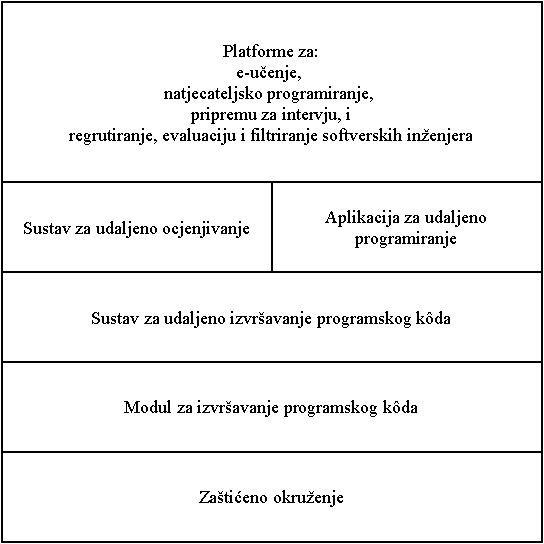
\includegraphics[width=0.6\textwidth]{images/Ekosustav.pdf}
	\caption{Arhitektura OJ ekosustava. \citep{9245310}}
\end{figure}
\end{frame}

%\begin{frame}[fragile]
%\frametitle{Arhitektura ekosustava sustava za udaljeno ocjenjivanje}
%\framesubtitle{Zaštićeno okruženje}
%\begin{lstlisting}[
%	caption={Ispravan C program s beskonačnim vremenom prevođenja.},
%	language=c
%]
%#include </dev/random>
%int main() {
%    return 0;
%}
%\end{lstlisting}
%\begin{lstlisting}[
%	caption={C program s beskonačnim grananjem novih procesa.},
%	language=c
%]
%#include <unistd.h>
%int main() {
%    while(1) {
%        fork();
%    }
%    return 0;
%}
%\end{lstlisting}
%\end{frame}

%\placelogofalse
%\begin{frame}
%\frametitle{Arhitektura ekosustava sustava za udaljeno ocjenjivanje}
%\framesubtitle{Modul za izvršavanje programskog kôda}
%\begin{figure}[htb]
%	\centering
%	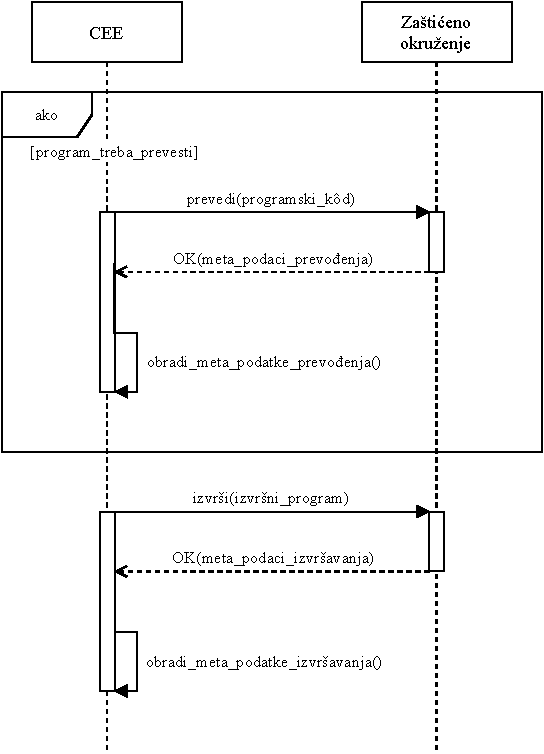
\includegraphics[width=0.42\textwidth]{images/CEE i zasticeno okruzenje.pdf}
%	\caption{
%		Interakcija modula za izvršavanje programskog kôda s zaštićenim okruženjem.
%	}
%\end{figure}
%\end{frame}
%\placelogotrue

%\placelogofalse
%\subsection{Sustav za udaljeno izvršavanje programskog kôda}
%\begin{frame}
%\frametitle{Arhitektura ekosustava sustava za udaljeno ocjenjivanje}
%\framesubtitle{Sustav za udaljeno izvršavanje programskog kôda}
%\begin{figure}[htb]
%	\centering
%	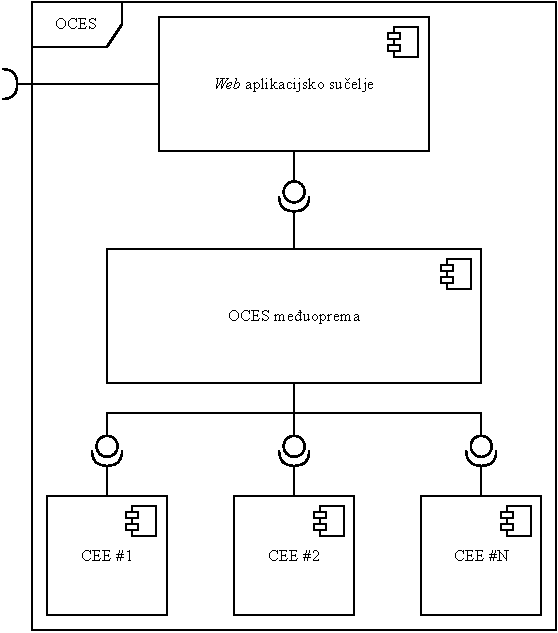
\includegraphics[width=0.5\textwidth]{images/Arhitektura OCES-a.pdf}
%	\caption{
%		Dijagram komponenti sustava za udaljeno izvršavanje programskog kôda.
%	}
%\end{figure}
%\end{frame}
%\placelogotrue

%\begin{frame}
%\frametitle{Sustav za udaljeno izvršavanje programskog kôda}
%\framesubtitle{Sustav Sphere Engine}
%\begin{figure}[htb]
%	\centering
%	
\includegraphics[width=0.75\textwidth]{images/Sphere Engine Logo.png}
%	\caption{
%		Vizualni identitet sustava Sphere Engine. \citep{SphereEngine}
%	}
%\end{figure}
%\end{frame}

%\begin{frame}
%\frametitle{Sustav za udaljeno izvršavanje programskog kôda}
%\framesubtitle{Sustav Piston}
%\begin{figure}[htb]
%	\centering
%	
\includegraphics[width=0.33\textwidth]{images/Piston Logo.png}
%	\caption{
%		Vizualni identitet sustava Piston. \citep{Piston}
%	}
%\end{figure}
%\end{frame}

%\begin{frame}
%\frametitle{Sustav za udaljeno izvršavanje programskog kôda}
%\framesubtitle{Sustav Judge0 (1)}
%\begin{figure}[htb]
%	\centering
%	
\includegraphics[width=0.66\textwidth]{images/Judge0 Logo.png}
%	\caption[]{
%		Vizualni identitet sustava Judge0.
%	}
%\end{figure}
%\end{frame}

%\placelogofalse
%\begin{frame}
%\frametitle{Sustav za udaljeno izvršavanje programskog kôda}
%\framesubtitle{Sustav Judge0 (2)}
%\begin{figure}[htb]
%	\centering
%	
\includegraphics[width=0.85\textwidth]{images/Judge0 Clients.png}
%	\caption{
%		Vizualni identiteti organizacija koje koriste sustav Judge0. \citep{Judge0Web}
%	}
%\end{figure}
%\end{frame}
%\placelogotrue

\begin{frame}
\frametitle{Arhitektura ekosustava sustava za udaljeno ocjenjivanje}
\framesubtitle{Sustav za udaljeno ocjenjivanje (1)}
\begin{figure}[htb]
	\centering
	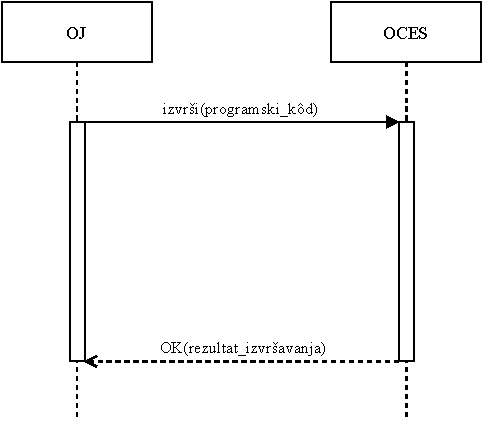
\includegraphics[width=0.75\textwidth]{images/Sync Interakcija.pdf}
	\caption{
		Sinkrona interakcija OJ-a i OCES-a.
	}
\end{figure}
\end{frame}

\begin{frame}
\frametitle{Arhitektura ekosustava sustava za udaljeno ocjenjivanje}
\framesubtitle{Sustav za udaljeno ocjenjivanje (2)}
\begin{figure}[htb]
	\centering
	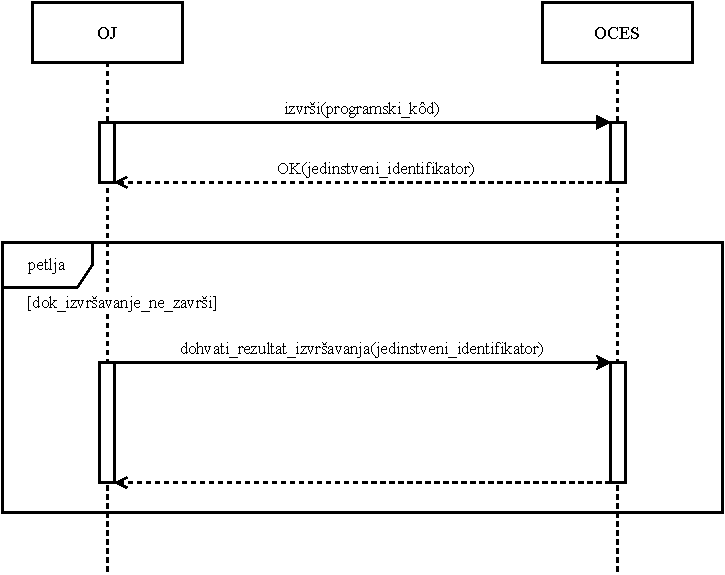
\includegraphics[width=0.7\textwidth]{images/Async Interakcija.pdf}
	\caption{
		Asinkrona interakcija OJ-a i OCES-a.
	}
\end{figure}
\end{frame}

%\placelogofalse
%\begin{frame}
%\frametitle{Arhitektura ekosustava sustava za udaljeno ocjenjivanje}
%\framesubtitle{\textit{Web} aplikacija za udaljeno programiranje}
%\begin{figure}[htb]
%	\centering
%	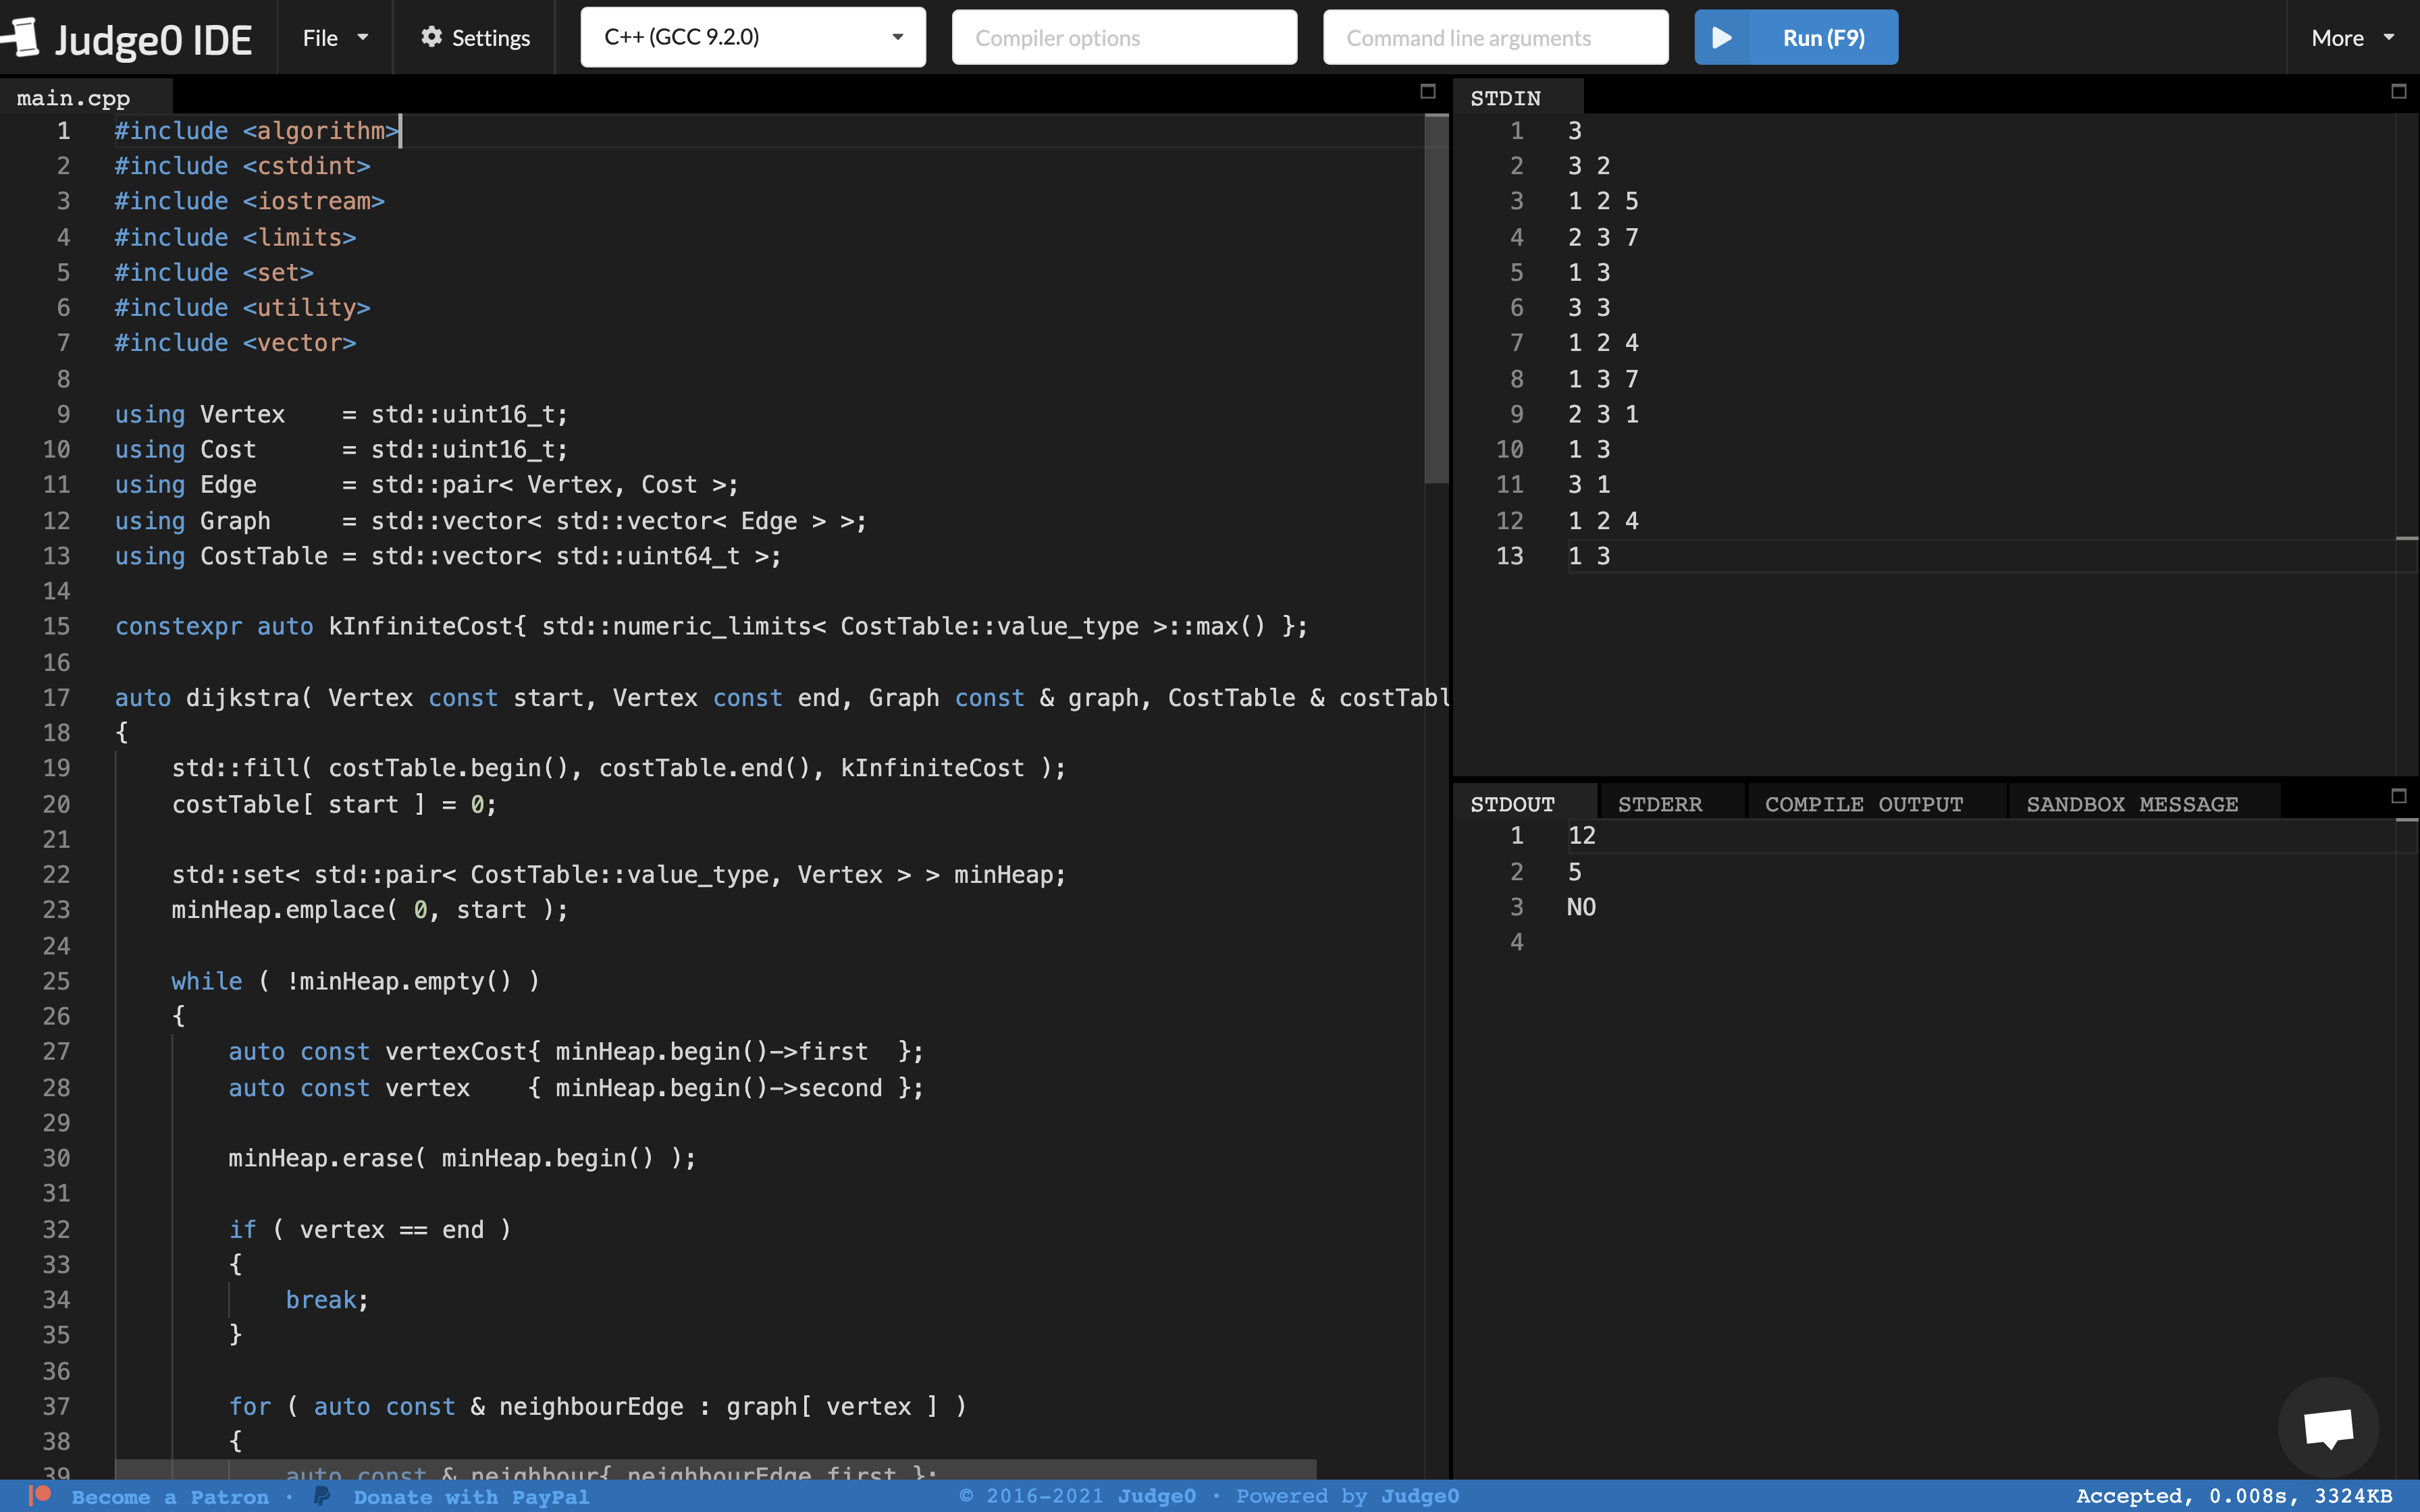
\includegraphics[width=0.9\textwidth]{images/Judge0 IDE UI.png}
%	\caption{
%		Sučelje \textit{web} aplikacije Judge0 IDE.
%	}
%\end{figure}
%\end{frame}
%\placelogotrue

%\placelogofalse
%\begin{frame}
%\frametitle{Arhitektura ekosustava sustava za udaljeno ocjenjivanje}
%\framesubtitle{Specijalizirane izvedbe sustava za udaljeno ocjenjivanje (1)}
%\begin{figure}[htb]
%	\centering
%	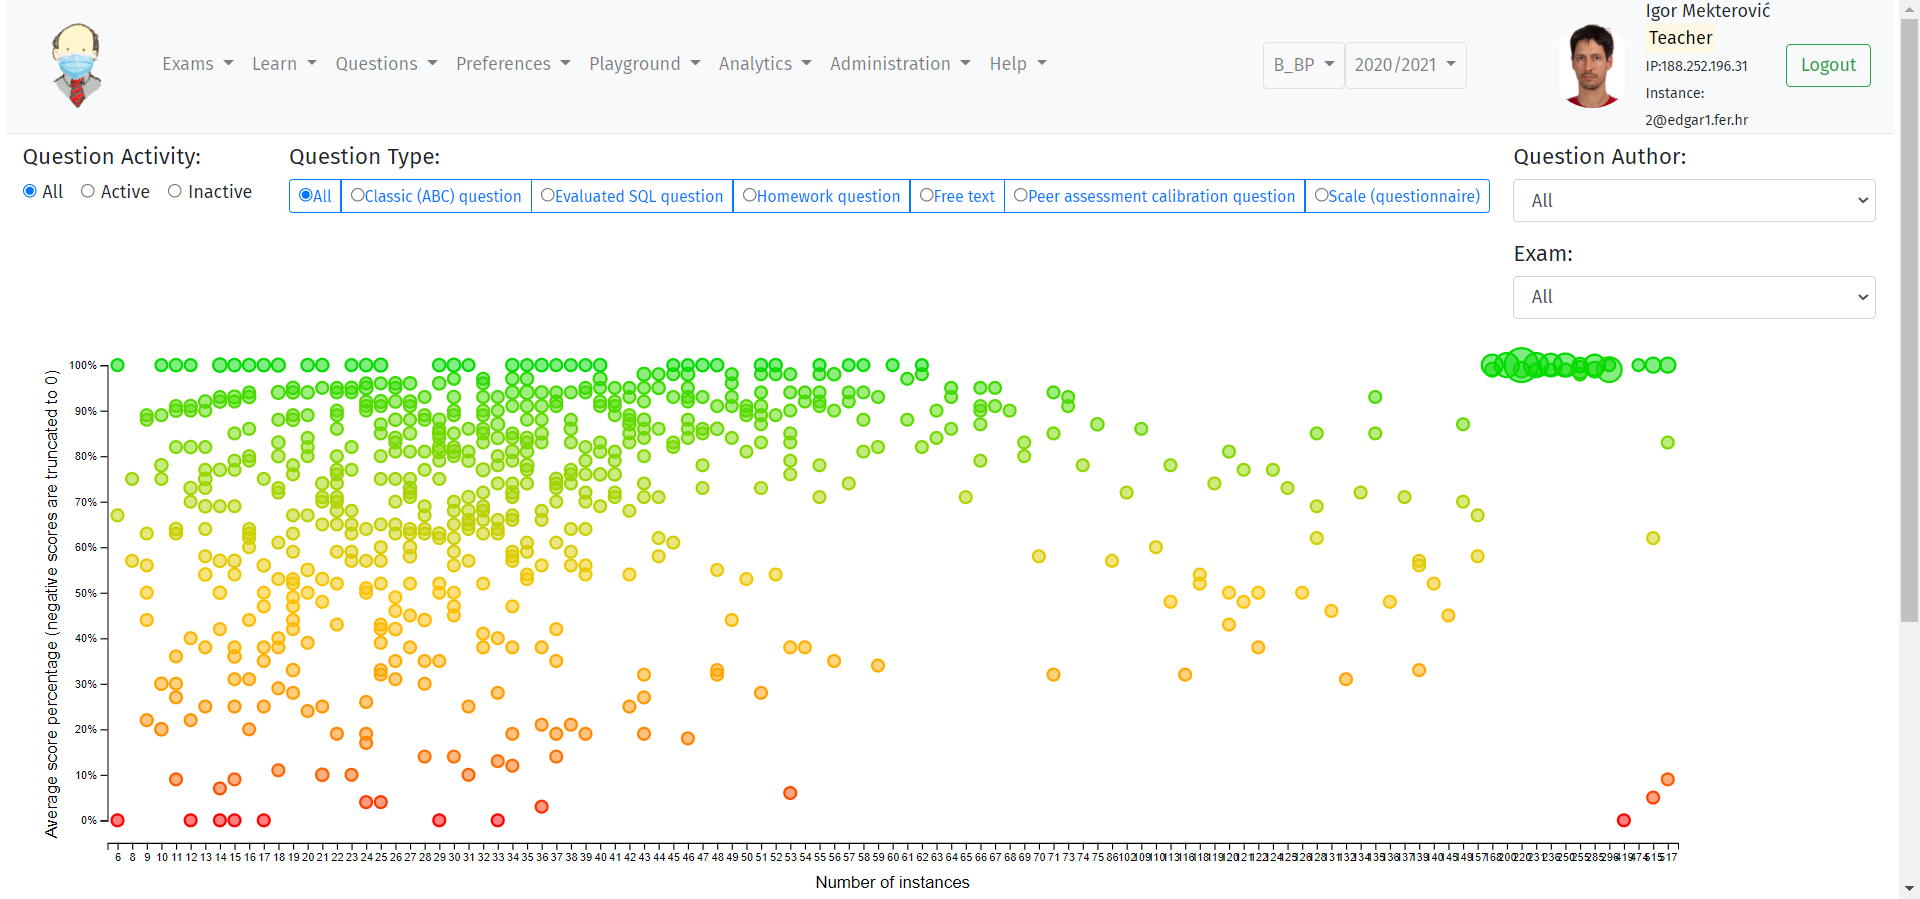
\includegraphics[width=\textwidth]{images/Edgar UI.png}
%	\caption{
%		Sučelje \textit{web} aplikacije Edgar iz perspektive učitelja.
%	}
%\end{figure}
%\end{frame}
%\placelogotrue

%\placelogofalse
%\begin{frame}
%\frametitle{Arhitektura ekosustava sustava za udaljeno ocjenjivanje}
%\framesubtitle{Specijalizirane izvedbe sustava za udaljeno ocjenjivanje (2)}
%\begin{figure}[htb]
%	\centering
%	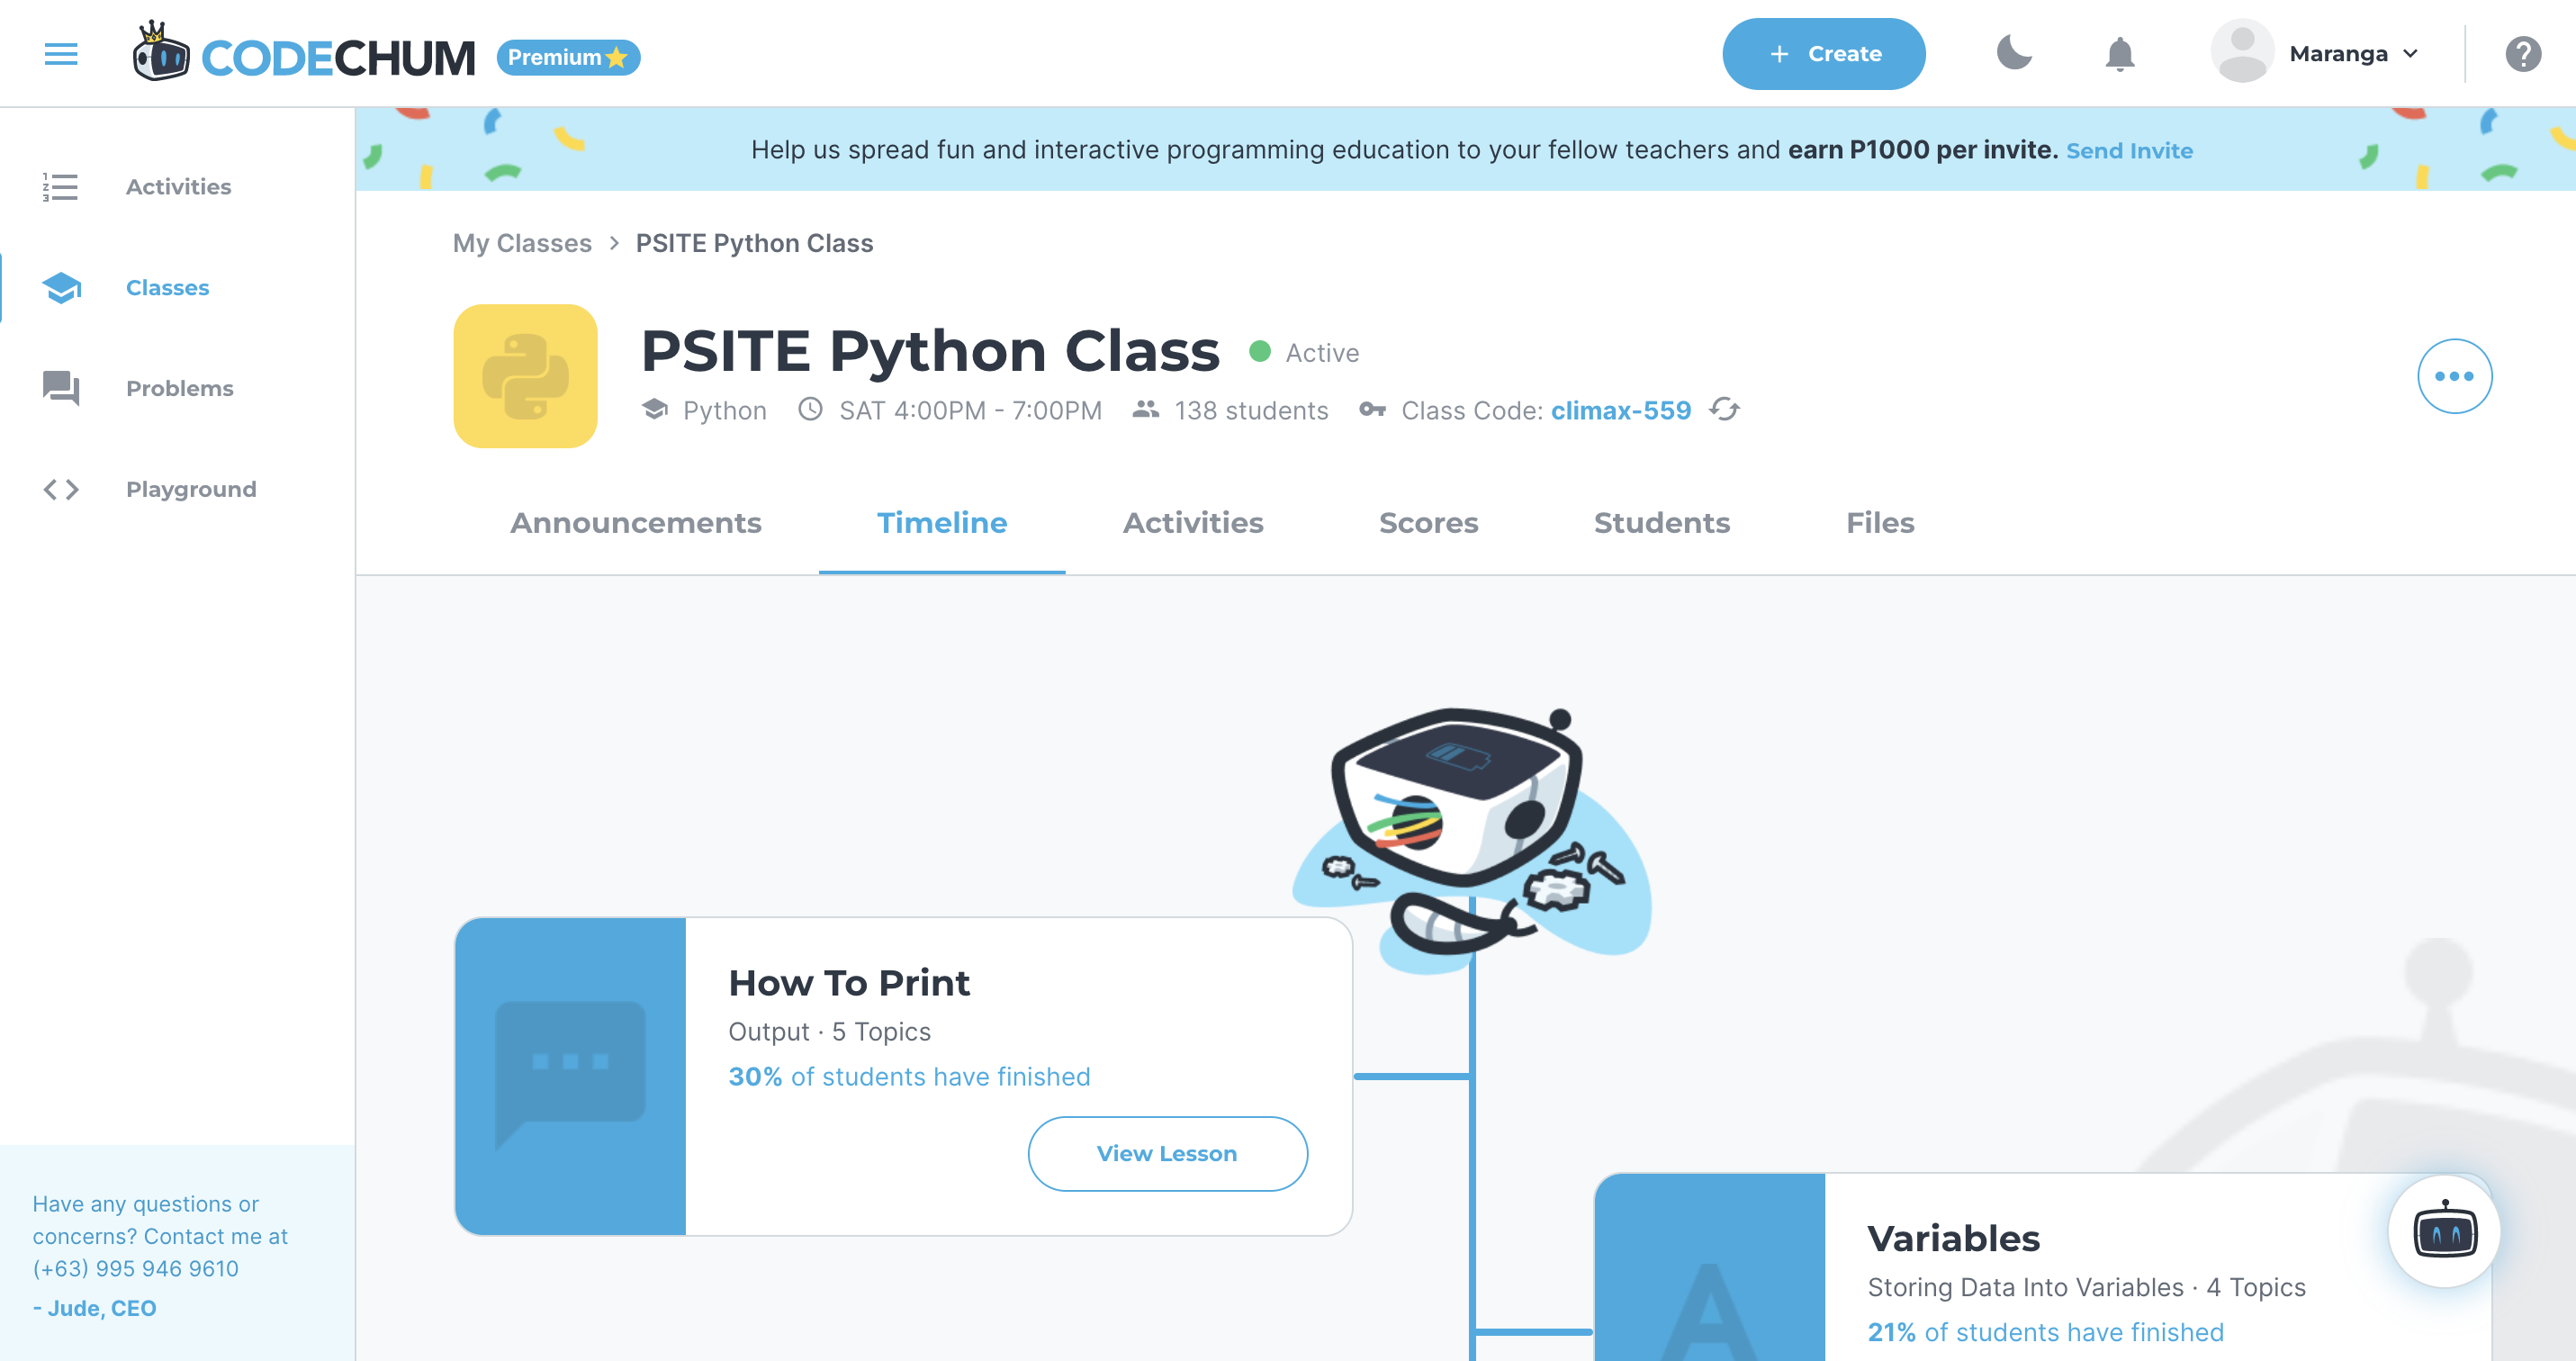
\includegraphics[width=\textwidth]{images/CodeChum UI.png}
%	\caption{
%		Sučelje \textit{web} aplikacije CodeChum.
%	}
%\end{figure}
%\end{frame}
%\placelogotrue

\section{Analiza performansi sustava za udaljeno izvršavanje programskog kôda}
\begin{frame}
\frametitle{Analiza performansi sustava za udaljeno izvršavanje programskog kôda}
\begin{itemize}
	\item dinamike višekorisničkog opterećenja
	\begin{itemize}
		\item impulsno-determinističko opterećenje
		\item kontinuirano-determinističko opterećenje
		\item kontinuirano-stohastičko opterećenje
	\end{itemize}
	\item scenariji korištenja
	\begin{itemize}
		\item jednostavan scenarij
		\item scenarij procesorskog opterećenja
		\item scenarij mrežnog opterećenja
		\item scenarij procesorskog i mrežnog opterećenja
	\end{itemize}
	\item metrike za analizu performansi
	\begin{itemize}
		\item uspješnost izvršavanja
		\item vrijeme obrade
		\item maksimalno opterećenje
	\end{itemize}
\end{itemize}
\end{frame}

%\placelogofalse
%\begin{frame}
%\frametitle{Analiza performansi sustava za udaljeno izvršavanje programskog kôda}
%\framesubtitle{Impulsno-determinističko opterećenje sustava}
%\begin{figure}[htb]
%	\centering
%	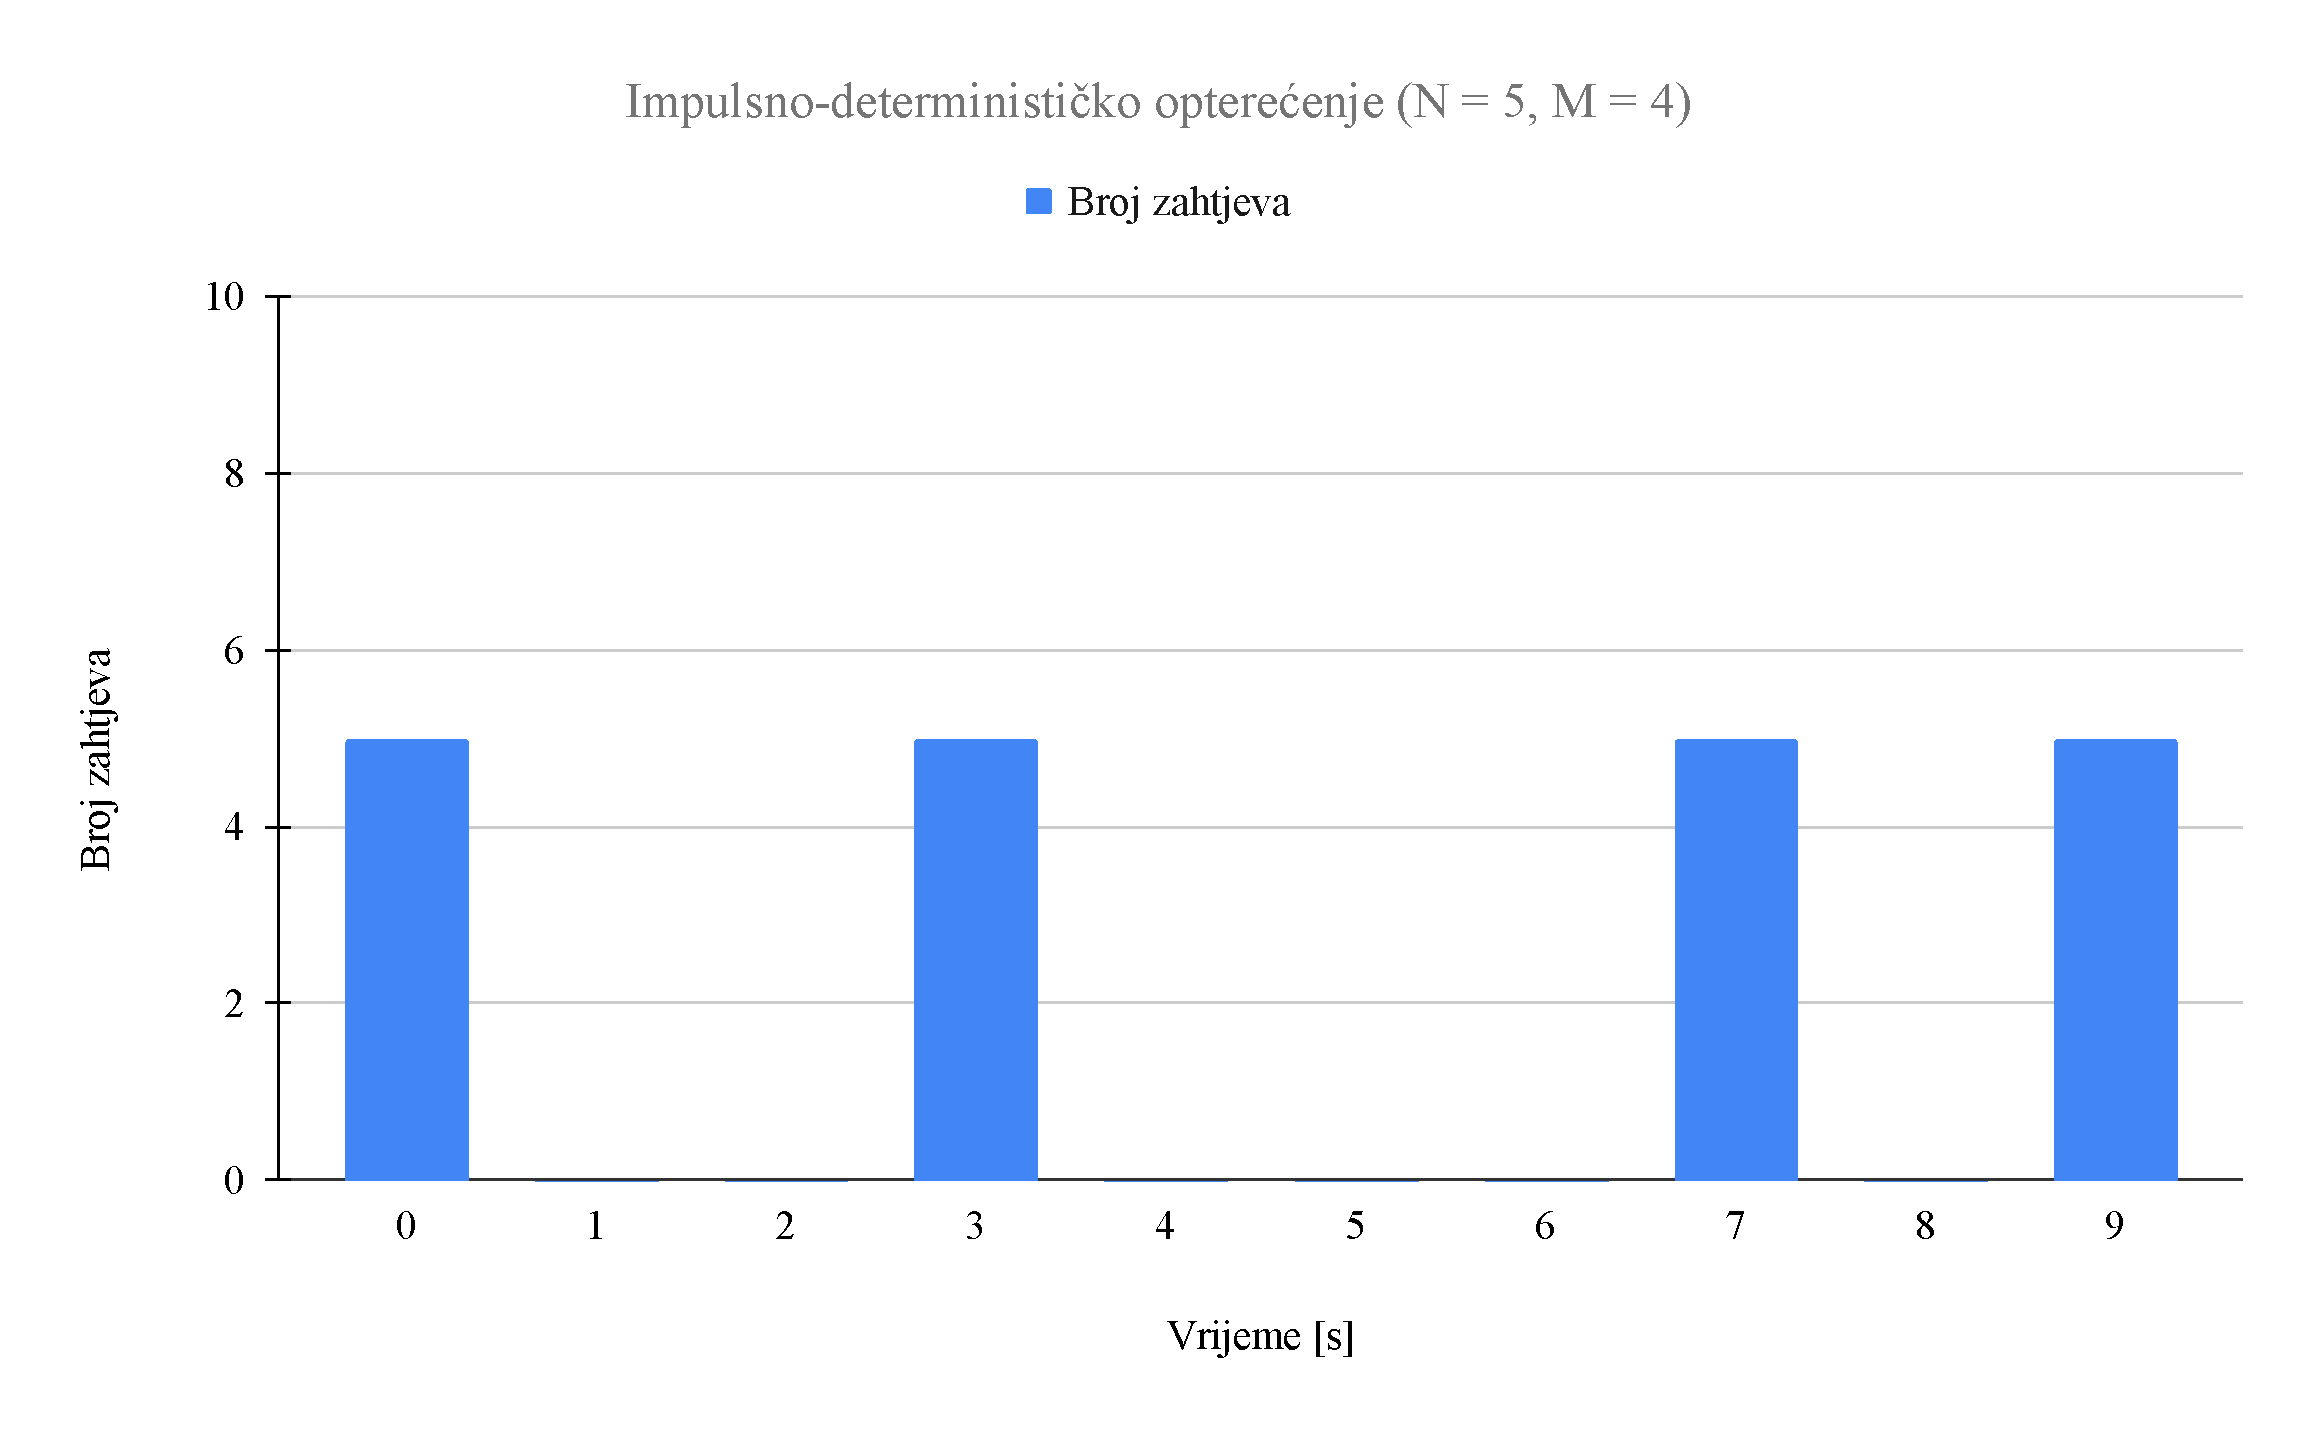
\includegraphics[width=0.8\textwidth]{images/Impulsno-deterministicko opterecenje (N = 5, M = 4).pdf}
%	\caption{
%		Impulsno-determinističko opterećenje sustava (N = 5, M = 4).
%	}
%\end{figure}
%\end{frame}
%\placelogotrue

%\placelogofalse
%\begin{frame}
%\frametitle{Analiza performansi sustava za udaljeno izvršavanje programskog kôda}
%\framesubtitle{Kontinuirano-determinističko opterećenje sustava}
%\begin{figure}[htb]
%	\centering
%	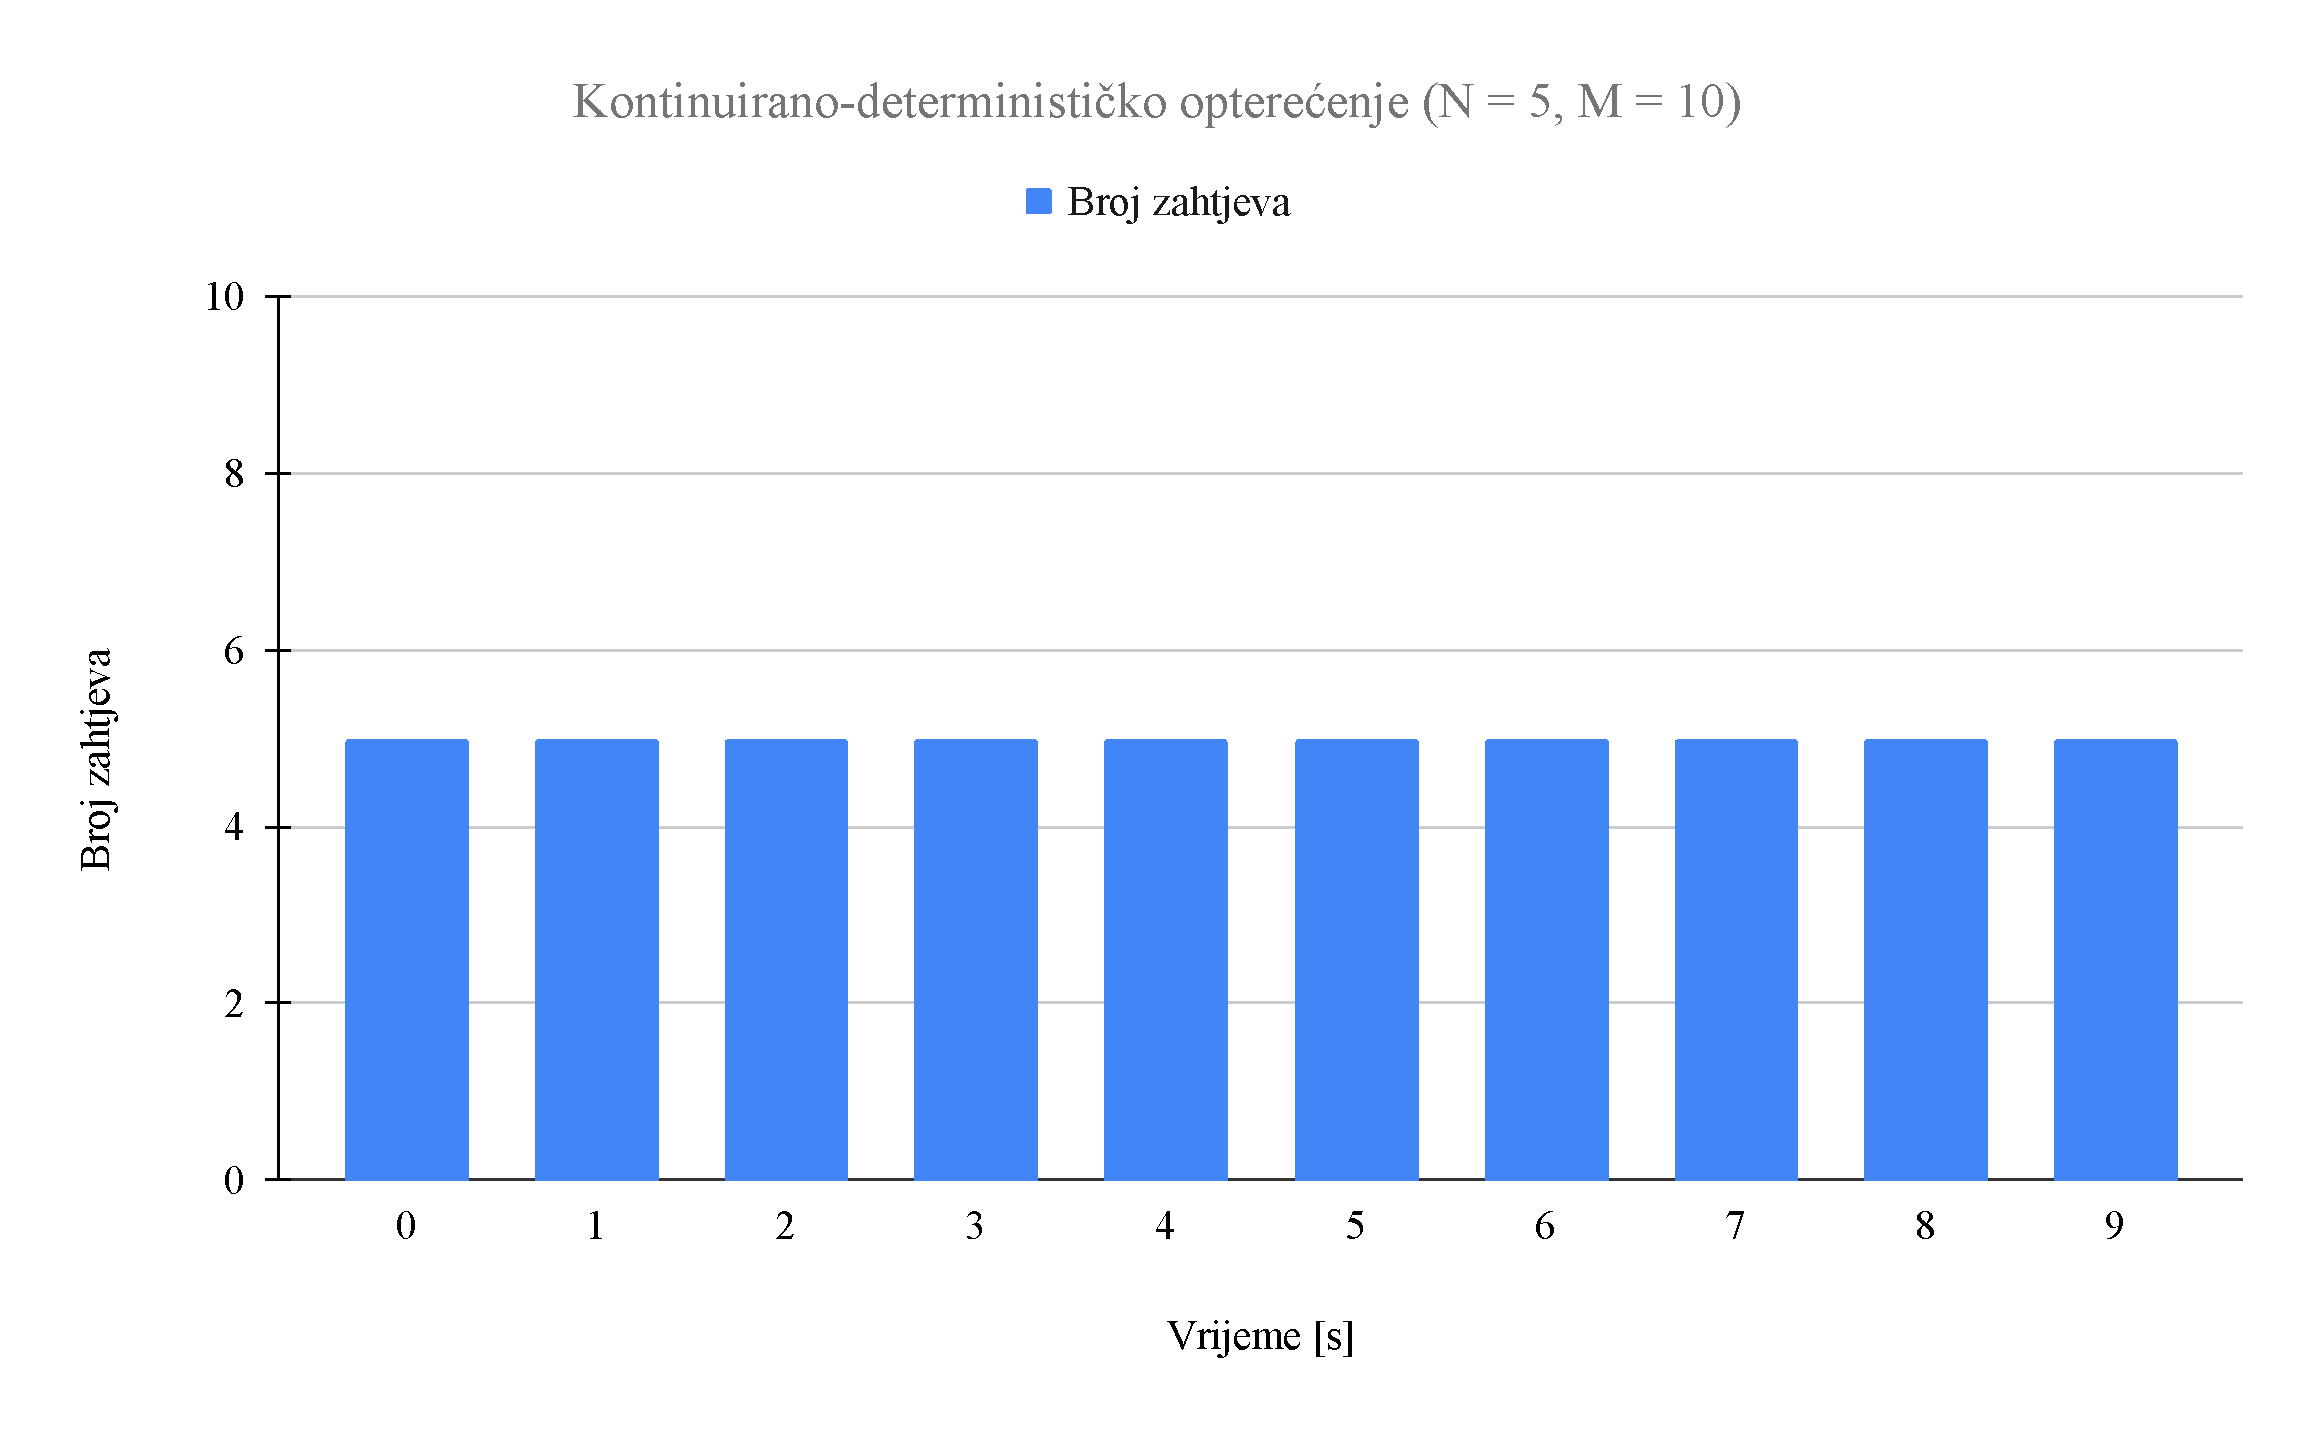
\includegraphics[width=0.8\textwidth]{images/Kontinuirano-deterministicko opterecenje (N = 5, M = 10).pdf}
%	\caption{
%		Kontinuirano-determinističko opterećenje sustava (N = 5, M = 10).
%	}
%\end{figure}
%\end{frame}
%\placelogotrue

\placelogofalse
\begin{frame}
\frametitle{Analiza performansi sustava za udaljeno izvršavanje programskog kôda}
\framesubtitle{Kontinuirano-stohastičko opterećenje sustava}
\begin{figure}[htb]
	\centering
	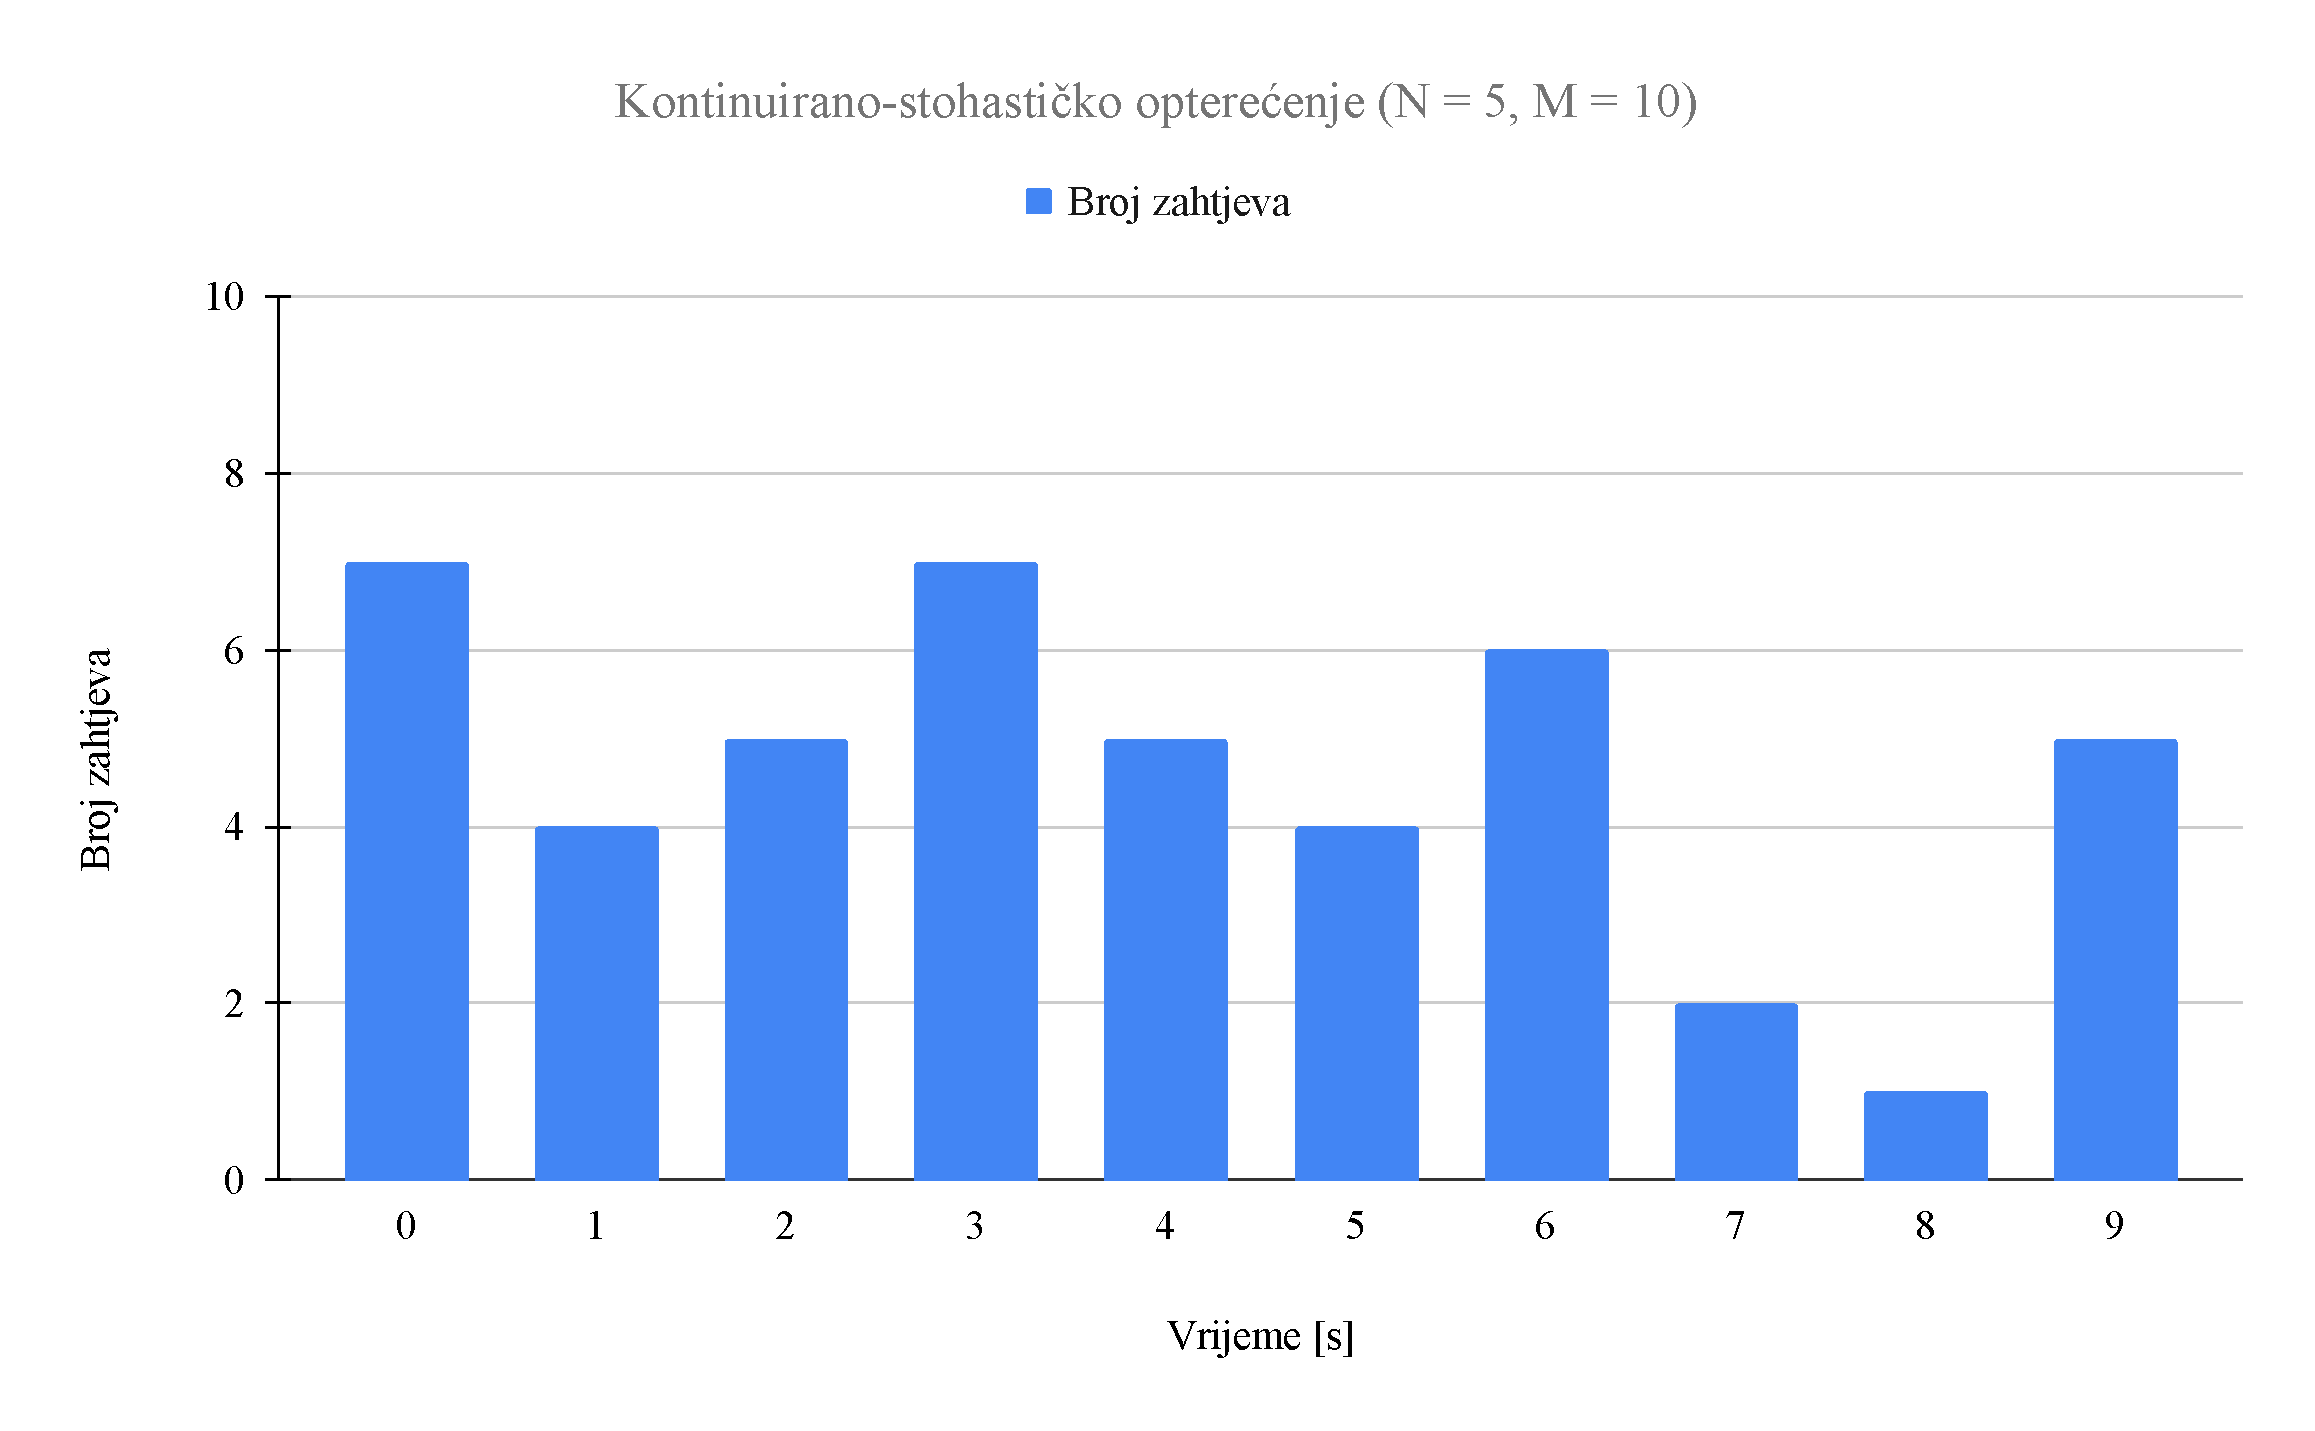
\includegraphics[width=0.8\textwidth]{images/Kontinuirano-stohasticko opterecenje (N = 5, M = 10).pdf}
	\caption{
		Kontinuirano-stohastičko opterećenje sustava (N = 5, M = 10).
	}
\end{figure}
\end{frame}
\placelogotrue

%\begin{frame}
%\frametitle{Analiza performansi sustava za udaljeno izvršavanje programskog kôda}
%\framesubtitle{Scenariji korištenja i programski jezici}
%Scenariji korištenja:
%\begin{itemize}
%	\item jednostavan scenarij
%	\item scenarij procesorskog opterećenja
%	\item scenarij mrežnog opterećenja
%	\item scenarij procesorskog i mrežnog opterećenja
%\end{itemize}
%
%\
%
%Programski jezici:
%\begin{itemize}
%	\item \text{C++}
%	\item Java
%	\item Python
%\end{itemize}
%\end{frame}

%\begin{frame}
%\frametitle{Analiza performansi sustava za udaljeno izvršavanje programskog kôda}
%\framesubtitle{Metrike za analizu performansi}
%\begin{itemize}
%	\item uspješnost izvršavanja
%	\item vrijeme obrade
%	\item maksimalno opterećenje
%\end{itemize}
%\end{frame}

\placelogofalse
\section{Aplikacija Hélory}
\begin{frame}[fragile]
\frametitle{Aplikacija Hélory}
\framesubtitle{Pregled komandno-linijskog sučelja}
\begin{lstlisting}[
	caption={Primjer pokretanja impulsno-determinističkog opterećenja.},
	numbers=none,
	xleftmargin=0cm,
	basicstyle=\scriptsize\ttfamily
]
$ ./helory run deterministic --users 5x10 \
                             --scenario hello_world \
                             --endpoint judge0_ce
\end{lstlisting}

\begin{lstlisting}[
	caption={Primjer pokretanja kontinuirano-determinističkog opterećenja.},
	numbers=none,
	xleftmargin=0cm,
	basicstyle=\scriptsize\ttfamily
]
$ ./helory run deterministic --users 5x10 --no-wait \
                             --scenario cpu_intensive \
                             --endpoint judge0_ce_fer
\end{lstlisting}

\begin{lstlisting}[
	caption={Primjer pokretanja kontinuirano-stohastičkog opterećenja.},
	numbers=none,
	xleftmargin=0cm,
	basicstyle=\scriptsize\ttfamily
]
$ ./helory run stochastic --intensity 5 --duration 10 \
                          --scenario cpu_and_network_intensive \
                          --endpoint piston_public
\end{lstlisting}
\end{frame}
\placelogotrue

\placelogofalse
\begin{frame}
\frametitle{Aplikacija Hélory}
\framesubtitle{Pregled sučelja grafičkog izvještaja (1)}
\begin{figure}[htb]
	\centering
	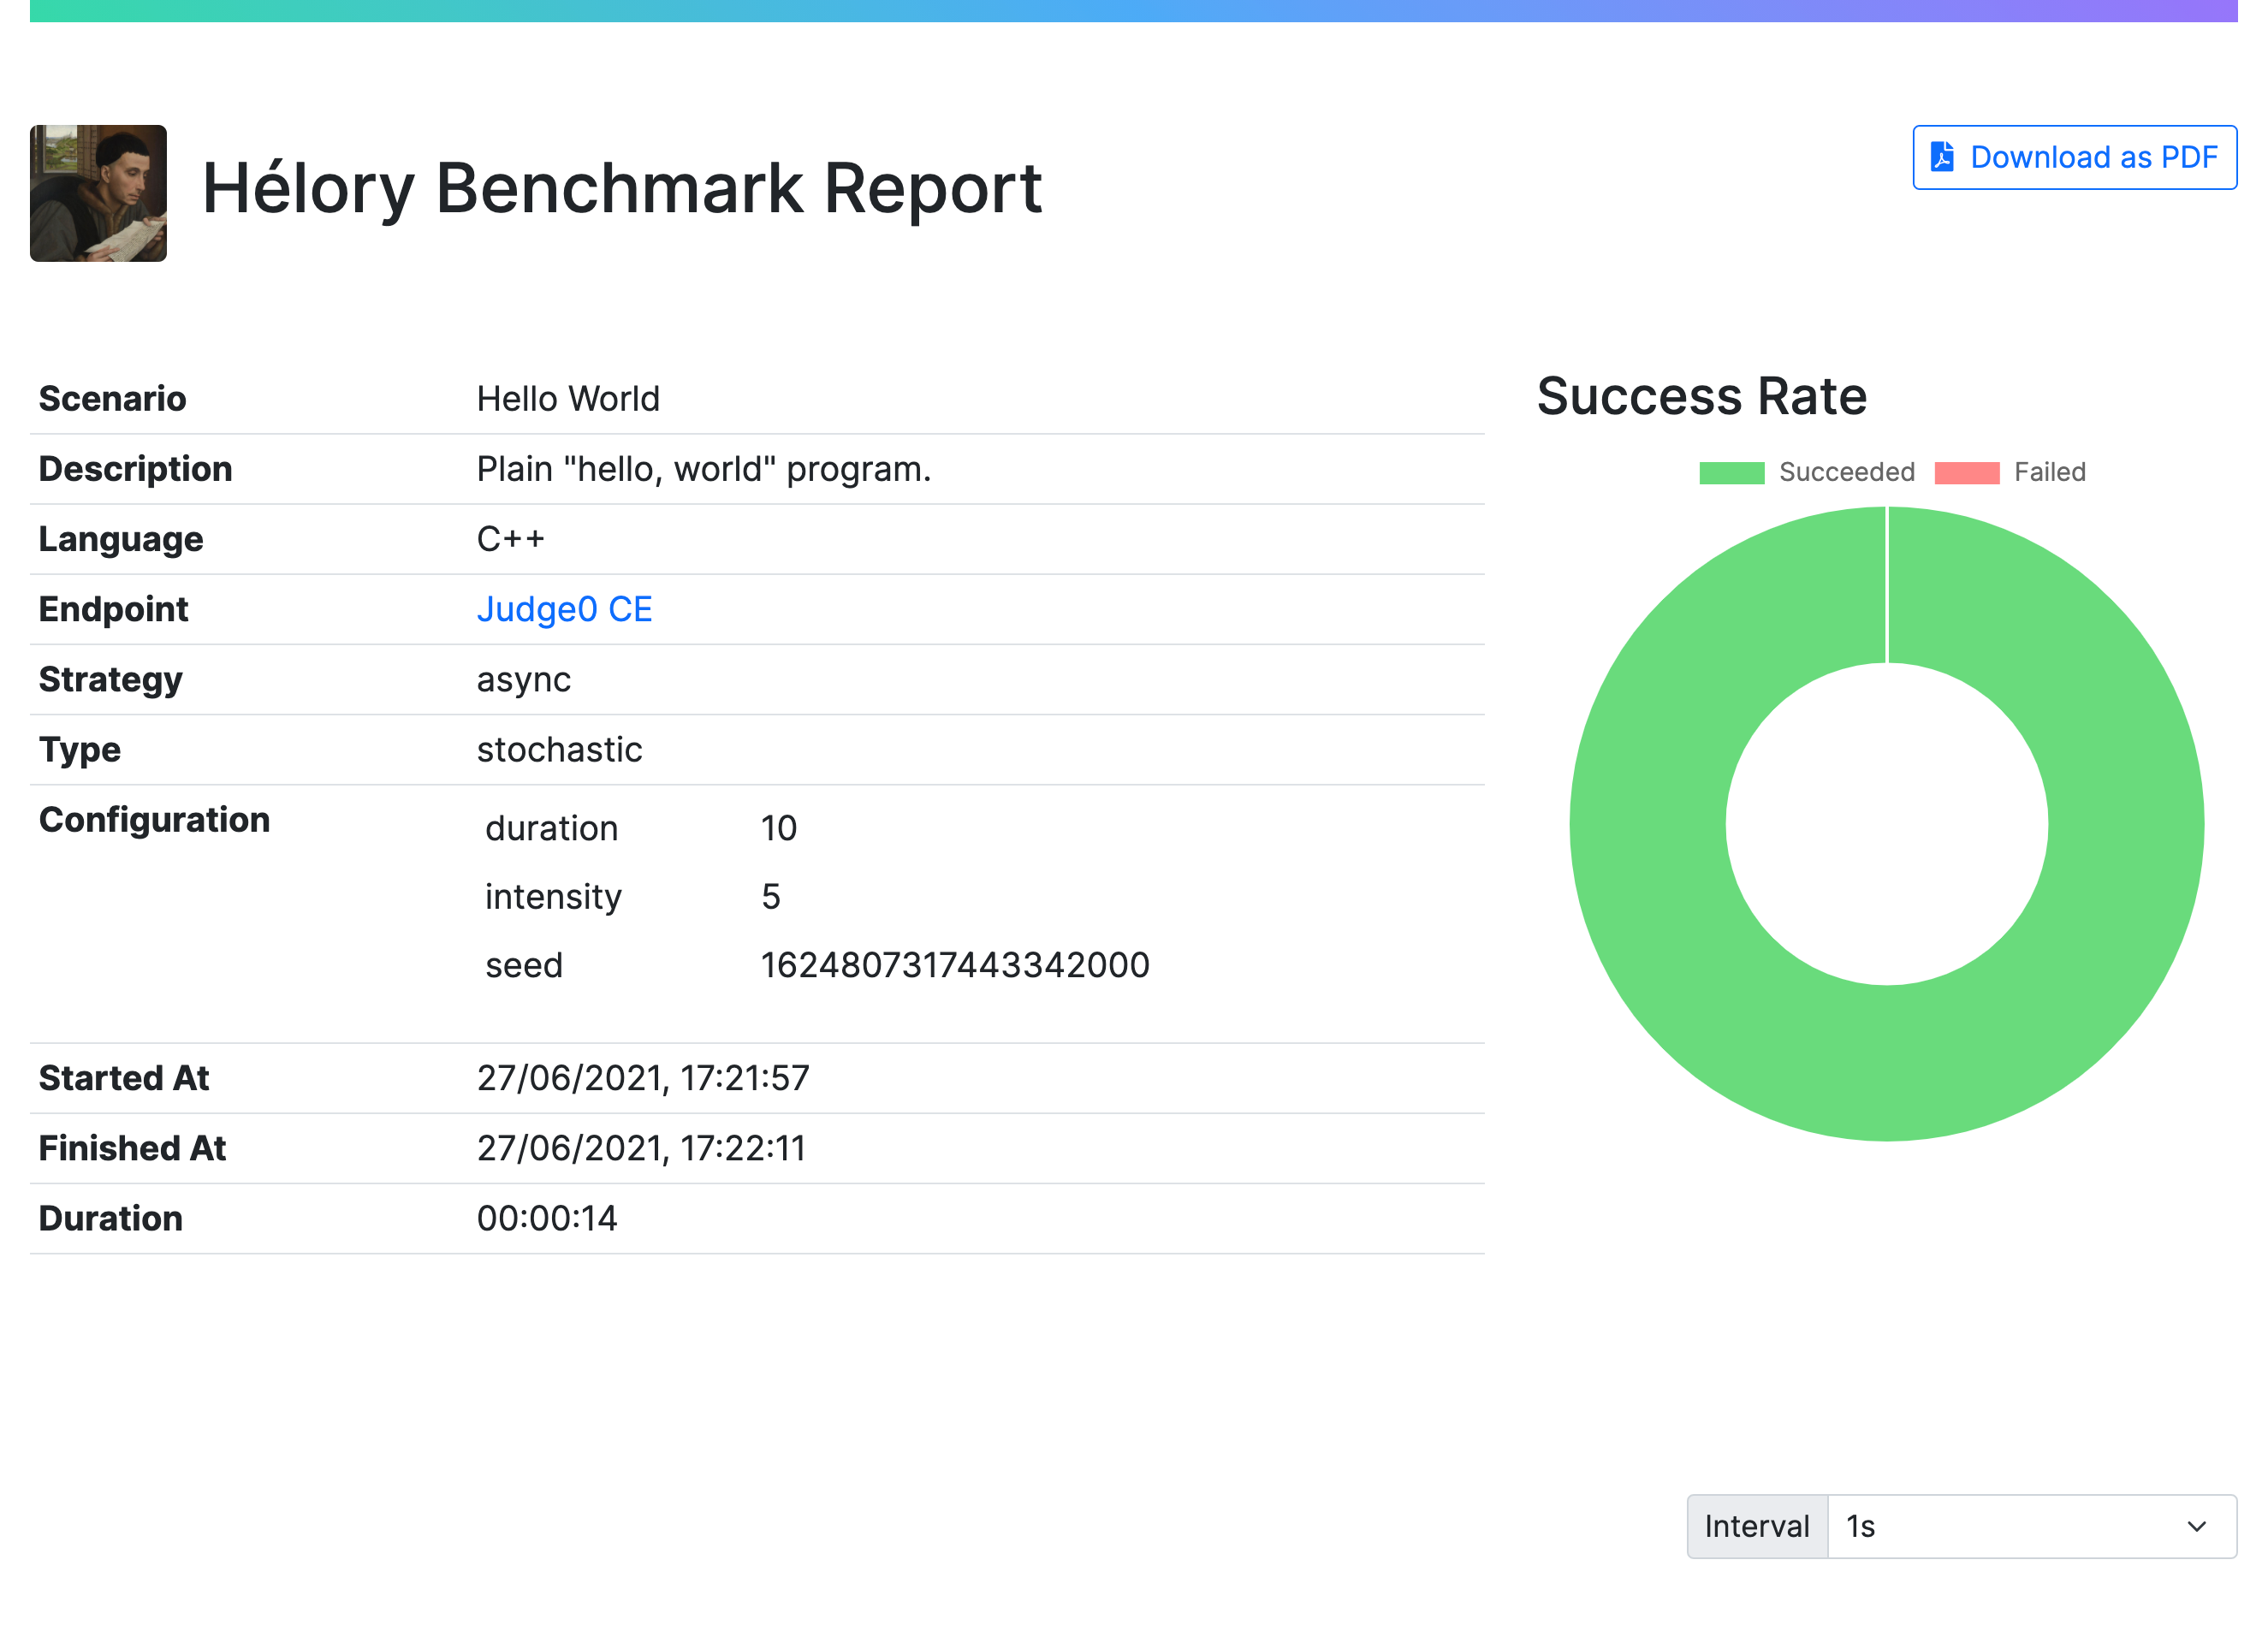
\includegraphics[width=0.8\textwidth]{images/Report UI 1.png}
	\caption{
		Prikaz detalja o pokrenutom eksperimentu.
	}
\end{figure}
\end{frame}
\placelogotrue

\placelogofalse
\begin{frame}
\frametitle{Aplikacija Hélory}
\framesubtitle{Pregled sučelja grafičkog izvještaja (2)}
\begin{figure}[htb]
	\centering
	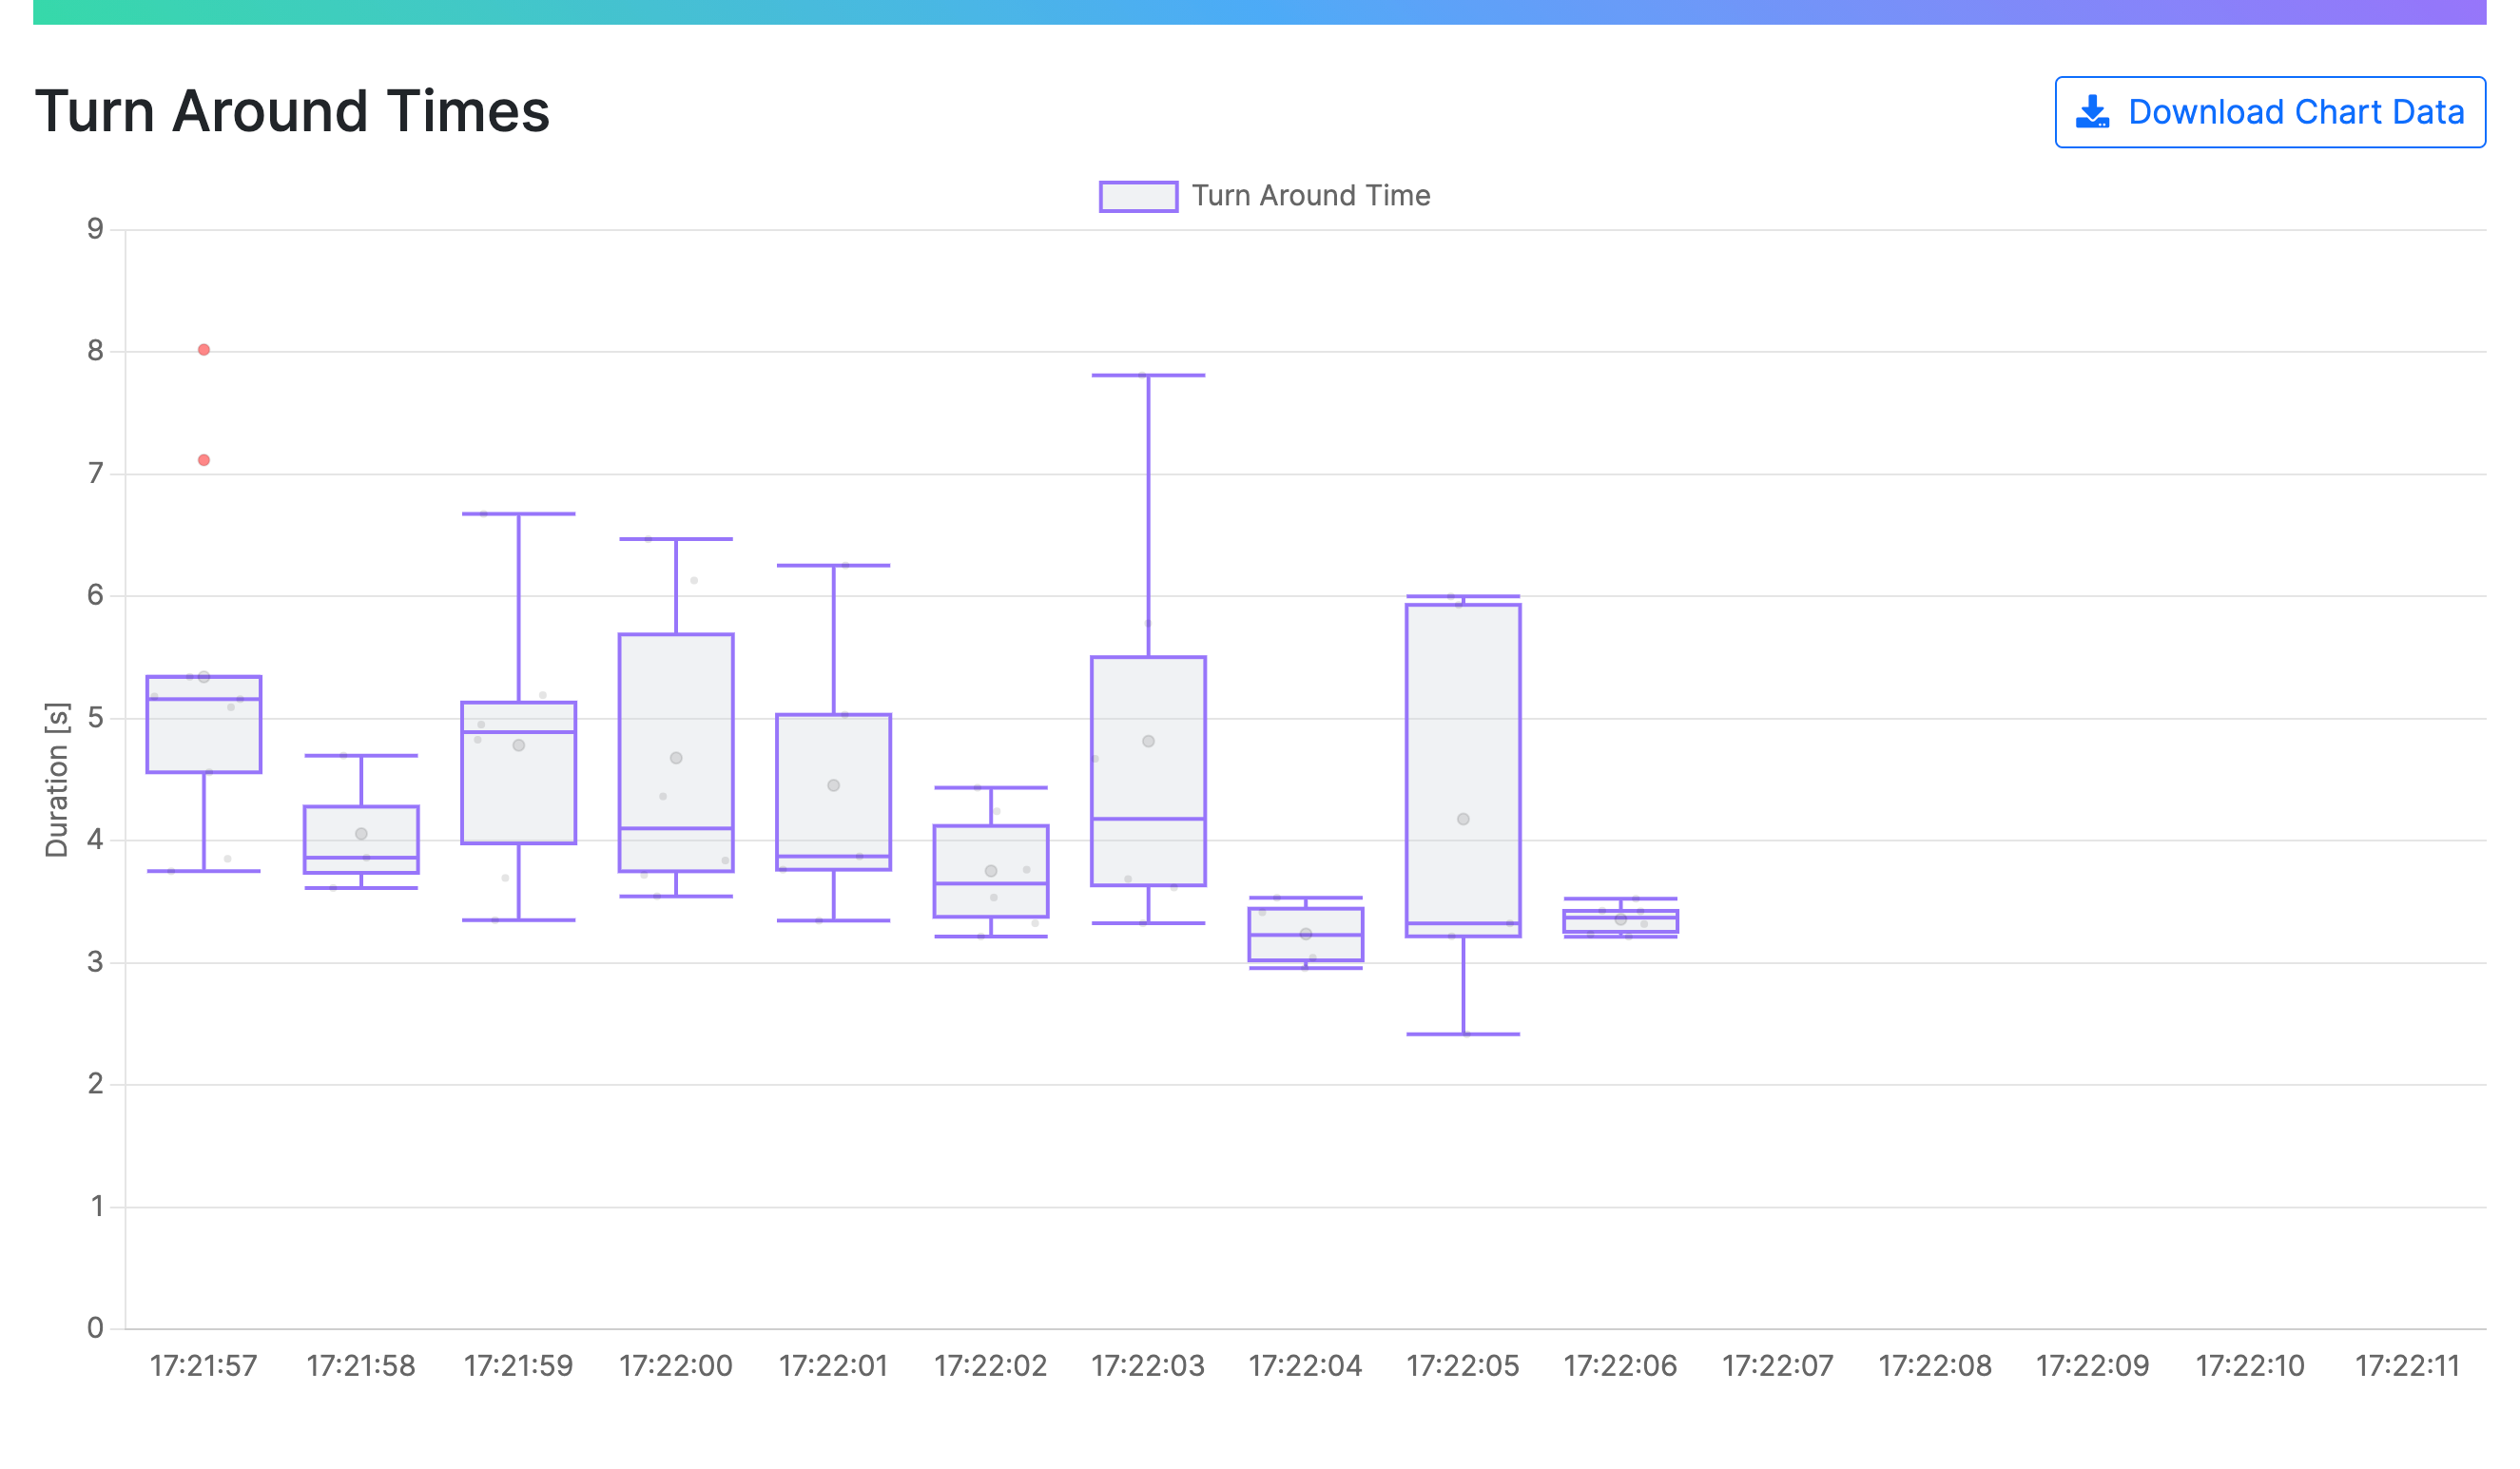
\includegraphics[width=0.9\textwidth]{images/Report UI 2.png}
	\caption{
		Prikaz dijagrama vremena obrade zahtjeva.
	}
\end{figure}
\end{frame}
\placelogotrue

\placelogofalse
\begin{frame}
\frametitle{Aplikacija Hélory}
\framesubtitle{Pregled sučelja grafičkog izvještaja (3)}
\begin{figure}[htb]
	\centering
	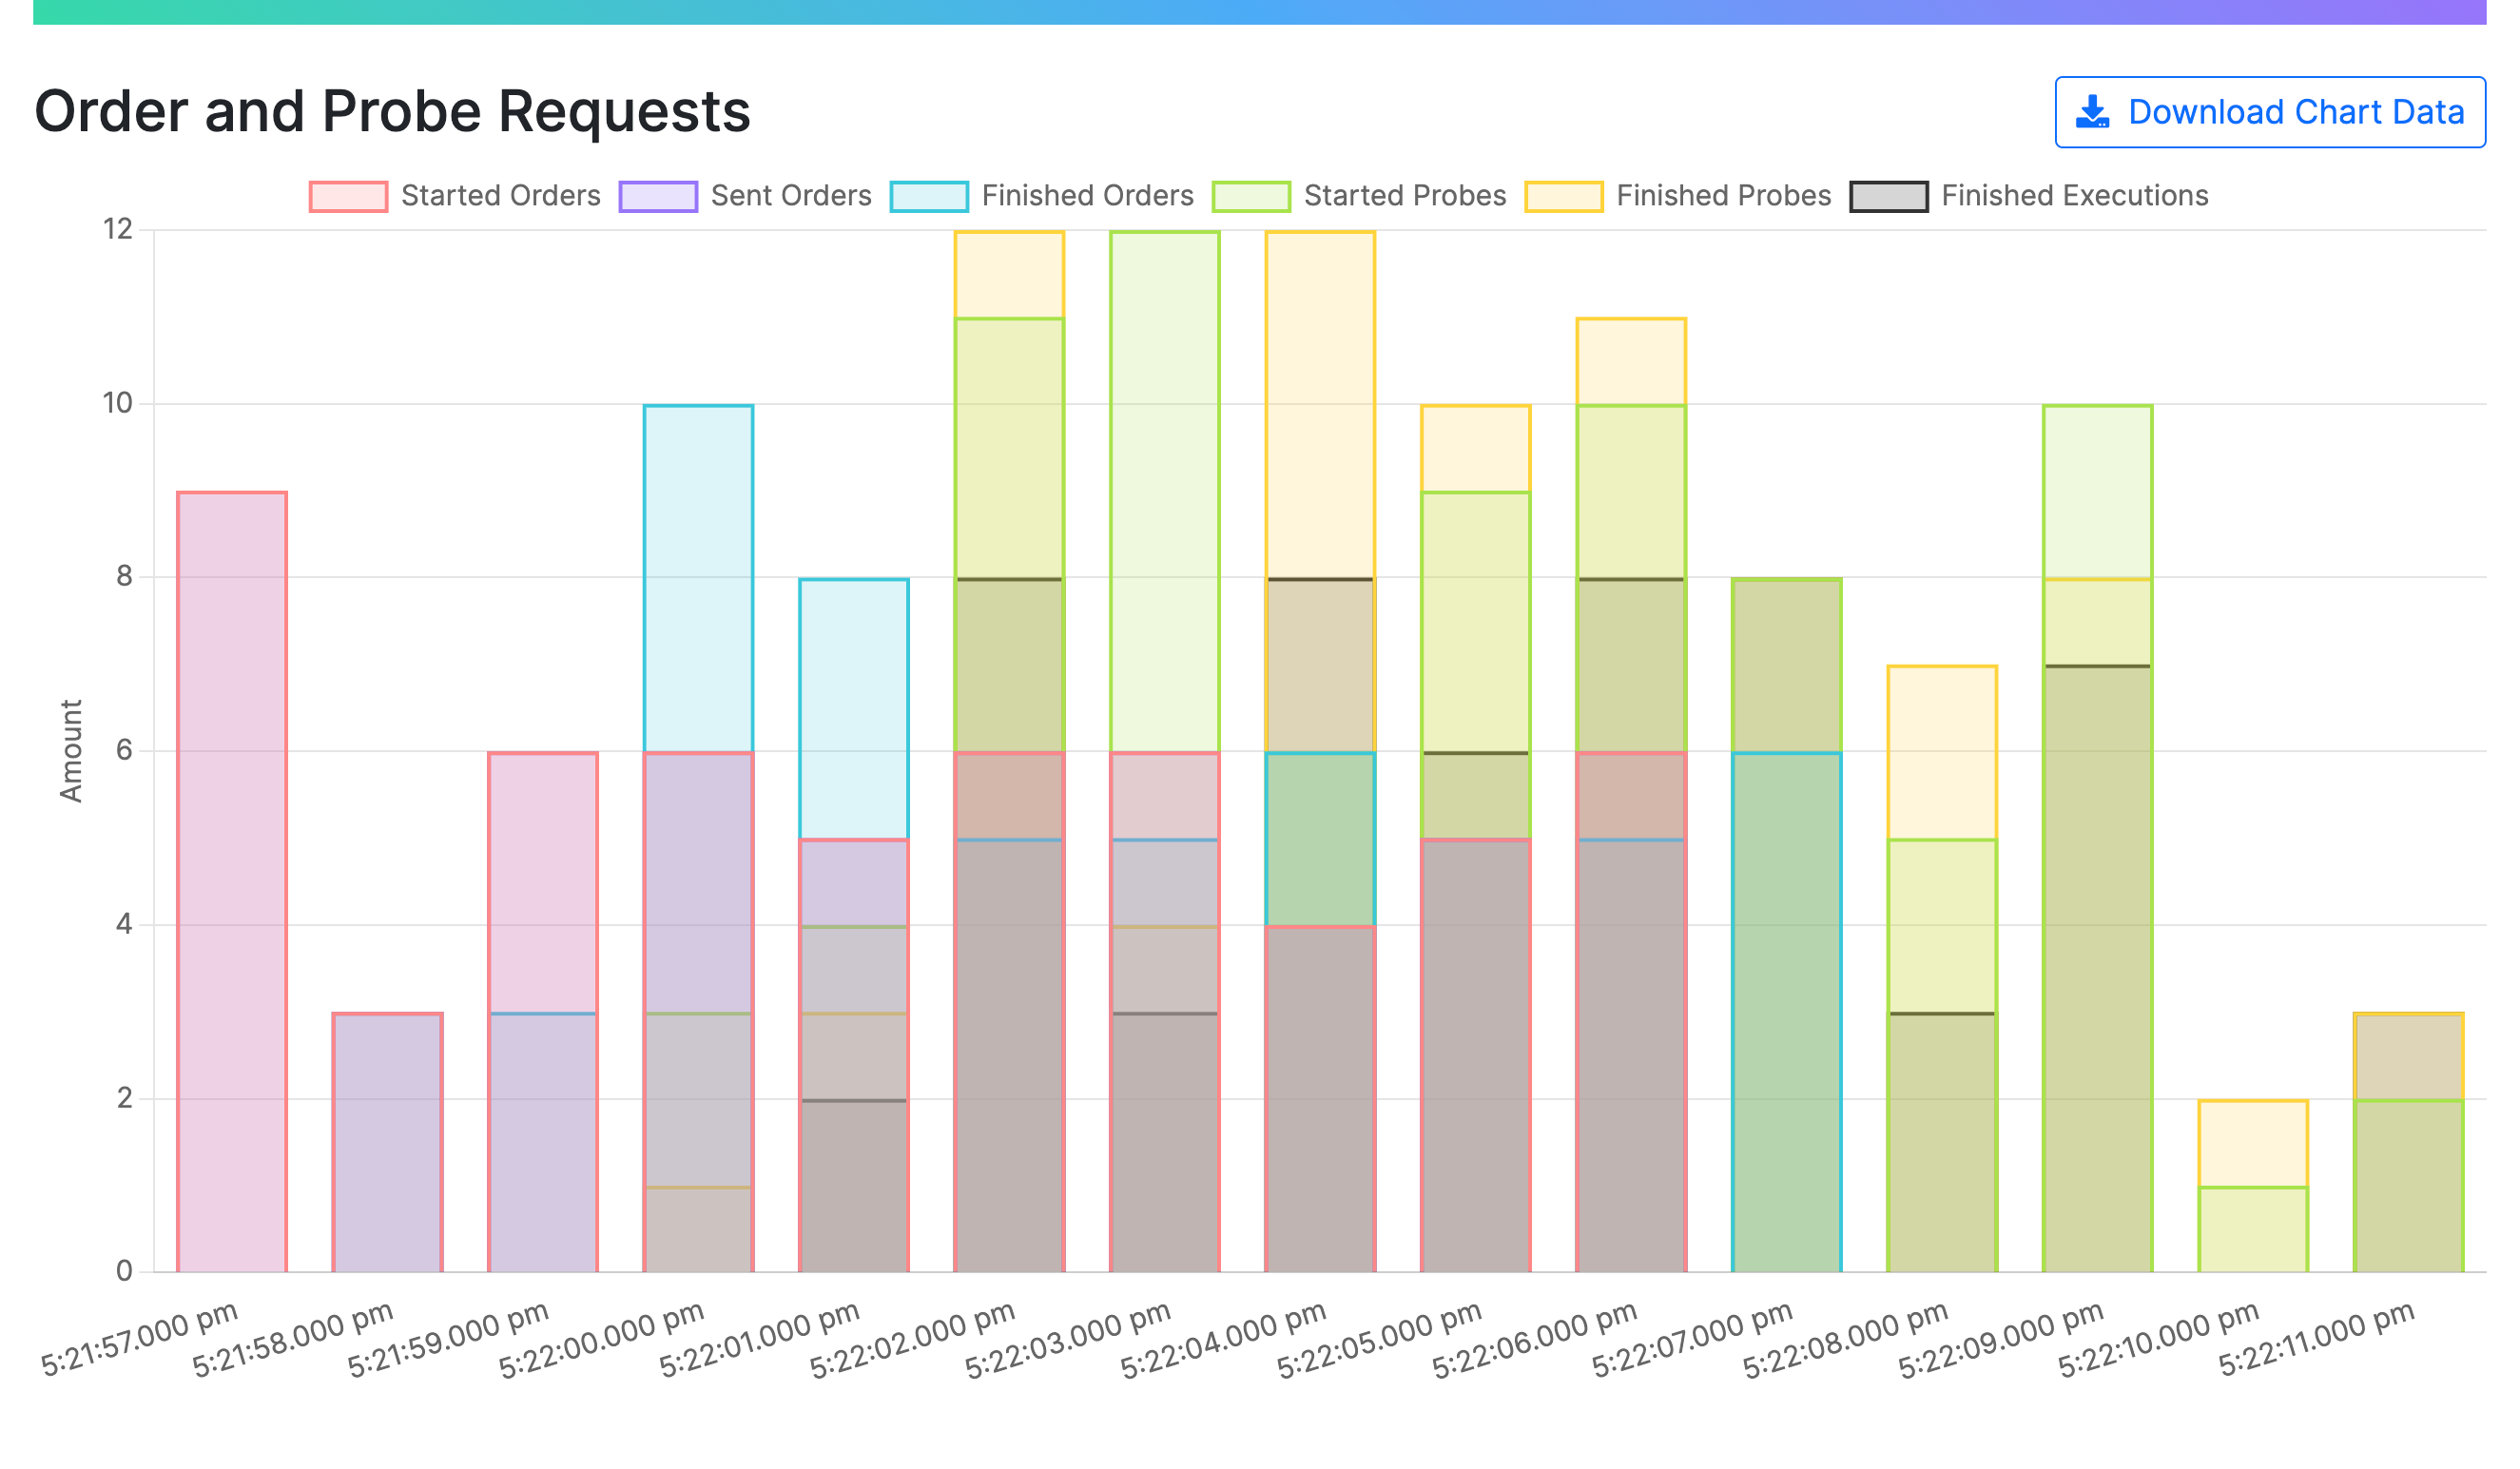
\includegraphics[width=0.9\textwidth]{images/Report UI 3.png}
	\caption{
		Prikaz grafa zahtjeva narudžbe i zahtjeva ispitivanja.
	}
\end{figure}
\end{frame}
\placelogotrue

\placelogofalse
\begin{frame}
\frametitle{Aplikacija Hélory}
\framesubtitle{Pregled sučelja grafičkog izvještaja (4)}
\begin{figure}[htb]
	\centering
	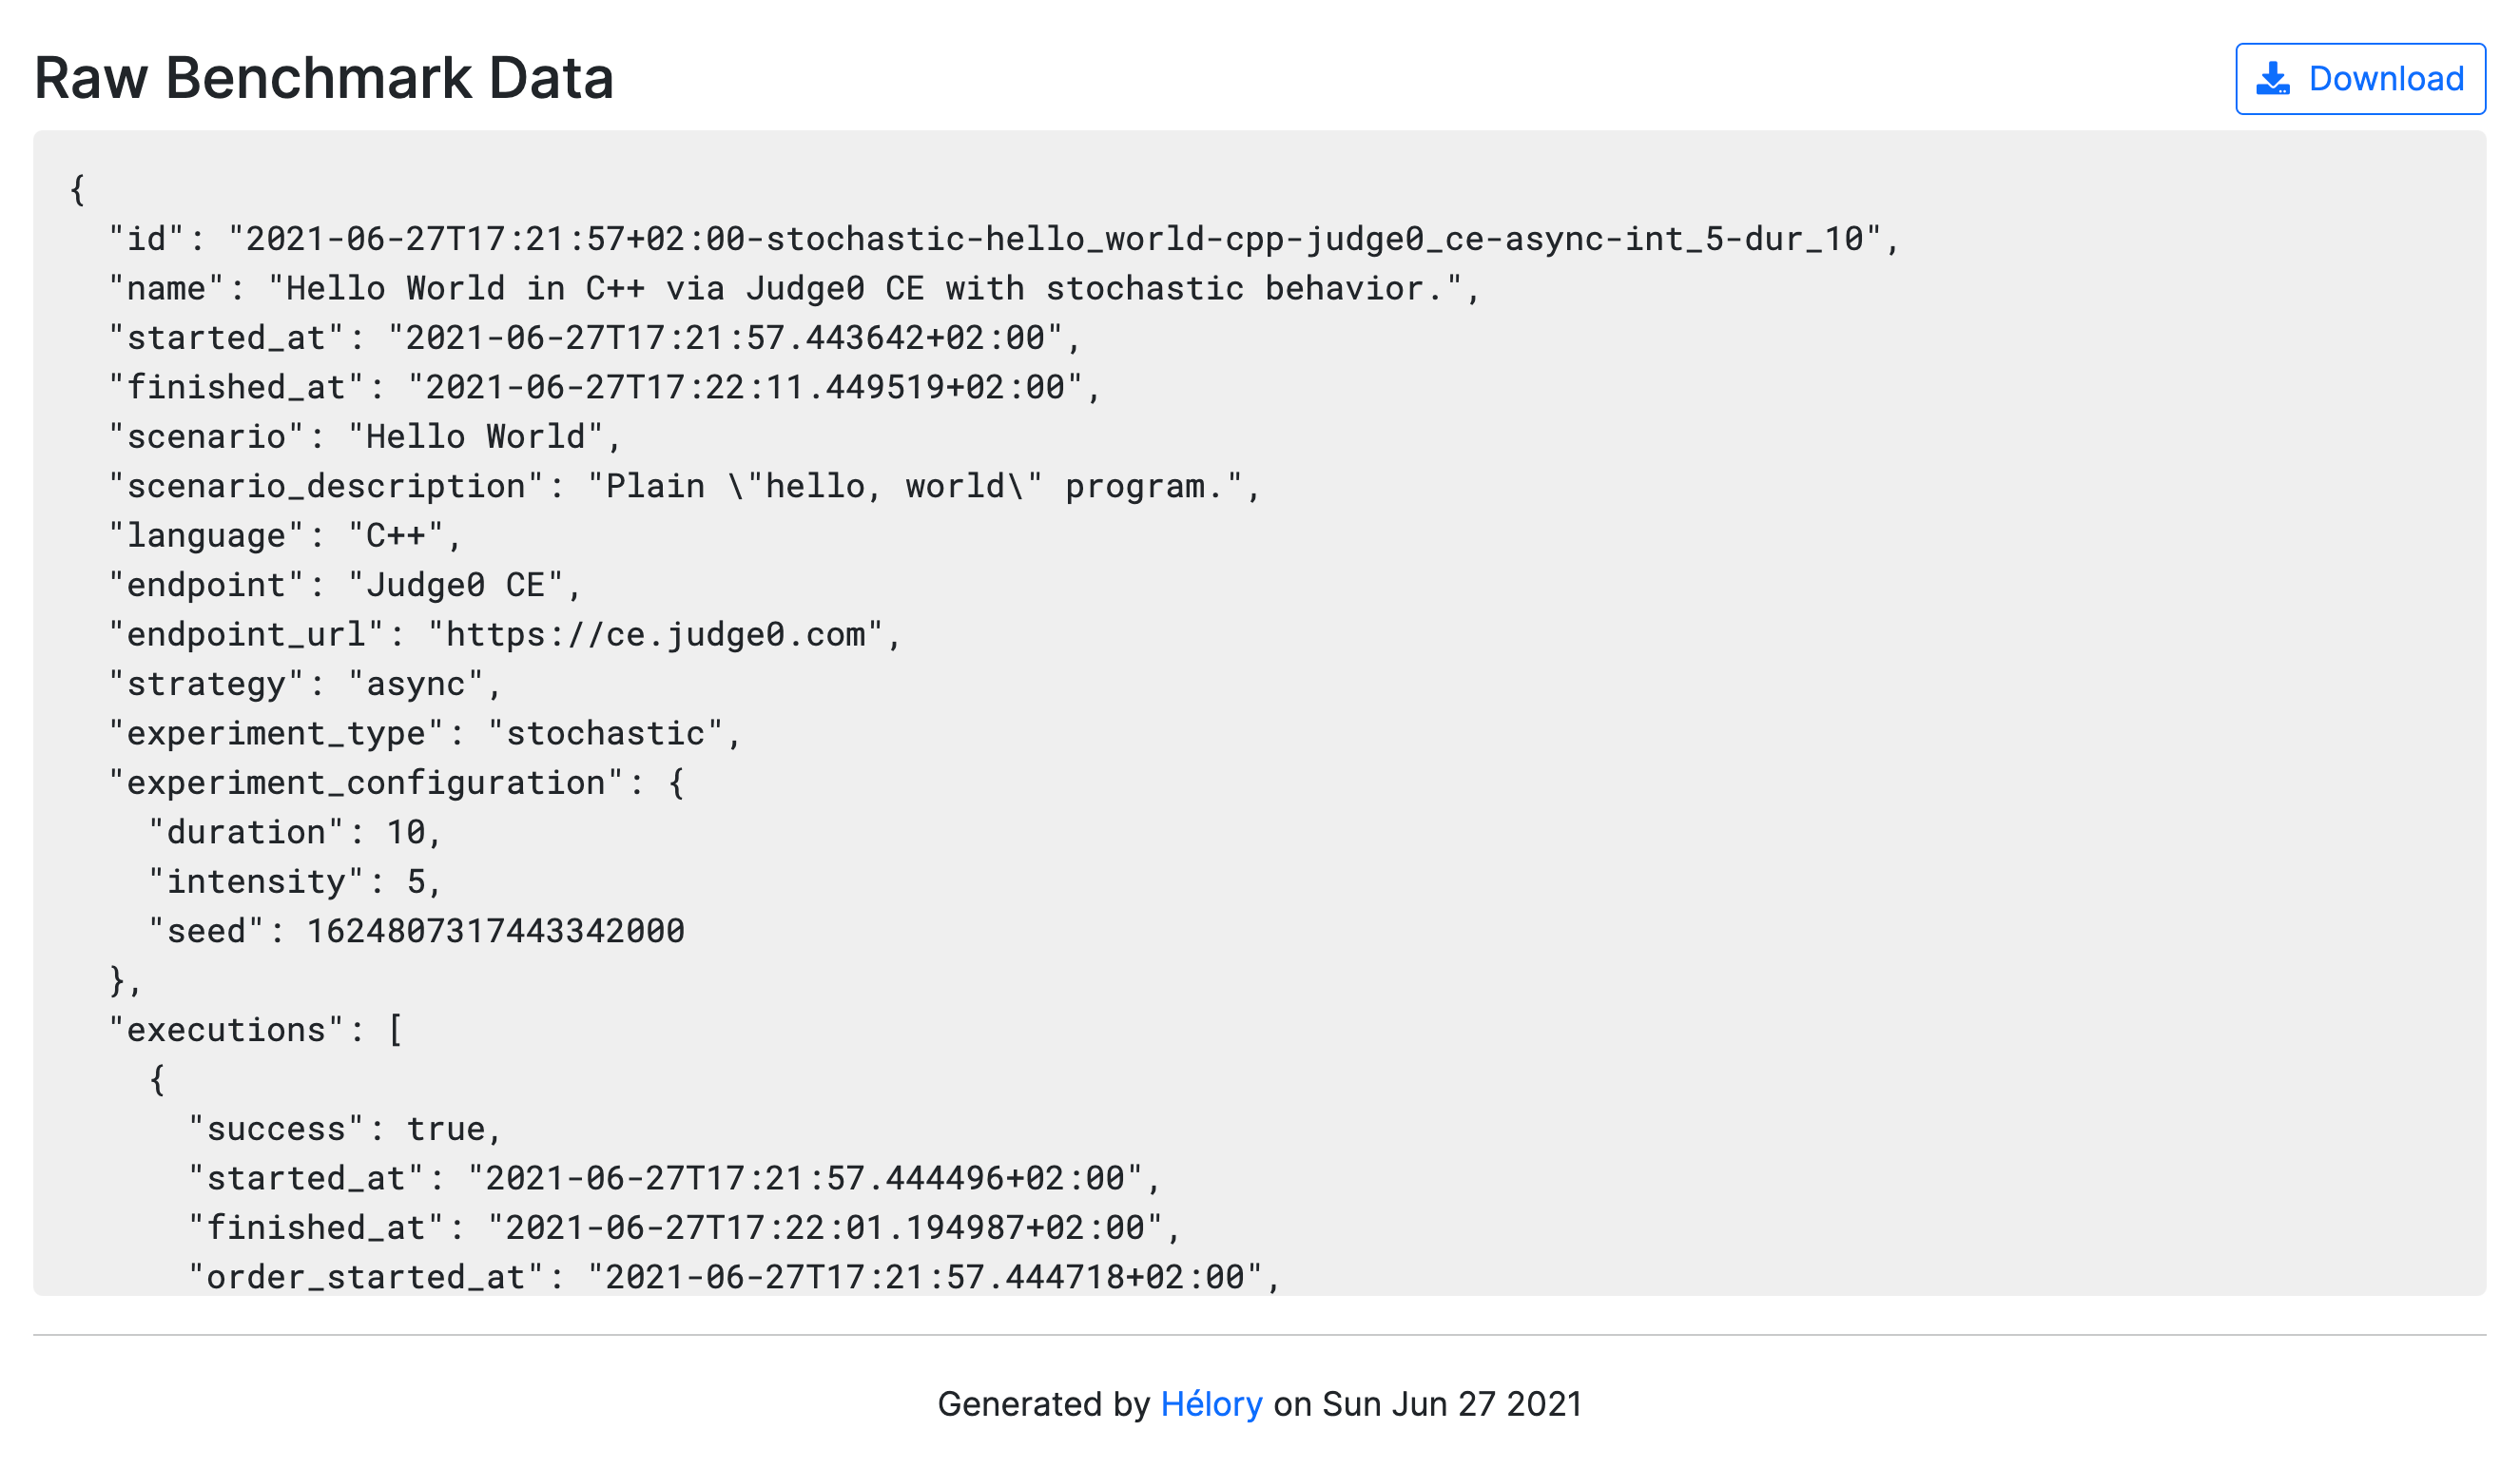
\includegraphics[width=\textwidth]{images/Report UI 4.png}
	\caption{
		Prikaz sirovih podatak prikupljenih za vrijeme eksperimenta.
	}
\end{figure}
\end{frame}
\placelogotrue

\section{Primjer korištenja aplikacije Hélory}
\begin{frame}
\frametitle{Primjer korištenja aplikacije Hélory}
\begin{itemize}
	\item $> 500$ eksperimenata
	\item FER-ova instanca sustava Judge0 
	\item kontinuirano-stohastičko opterećenje
	\begin{itemize}
		\item $N \in \left\{1,5,10,15,20,25\right\}$
		\item $M=60$
	\end{itemize}
	\item jednostavan scenarij korištenja
	\item sinkrona i asinkrona interakcija
	\item \text{C++}, Java i Python
\end{itemize}
\end{frame}

\placelogofalse
\begin{frame}
\frametitle{Primjer korištenja aplikacije Hélory}
\framesubtitle{Analiza performansi FER-ove instance sustava Judge0 (1)}
\begin{figure}[htb]
	\centering
	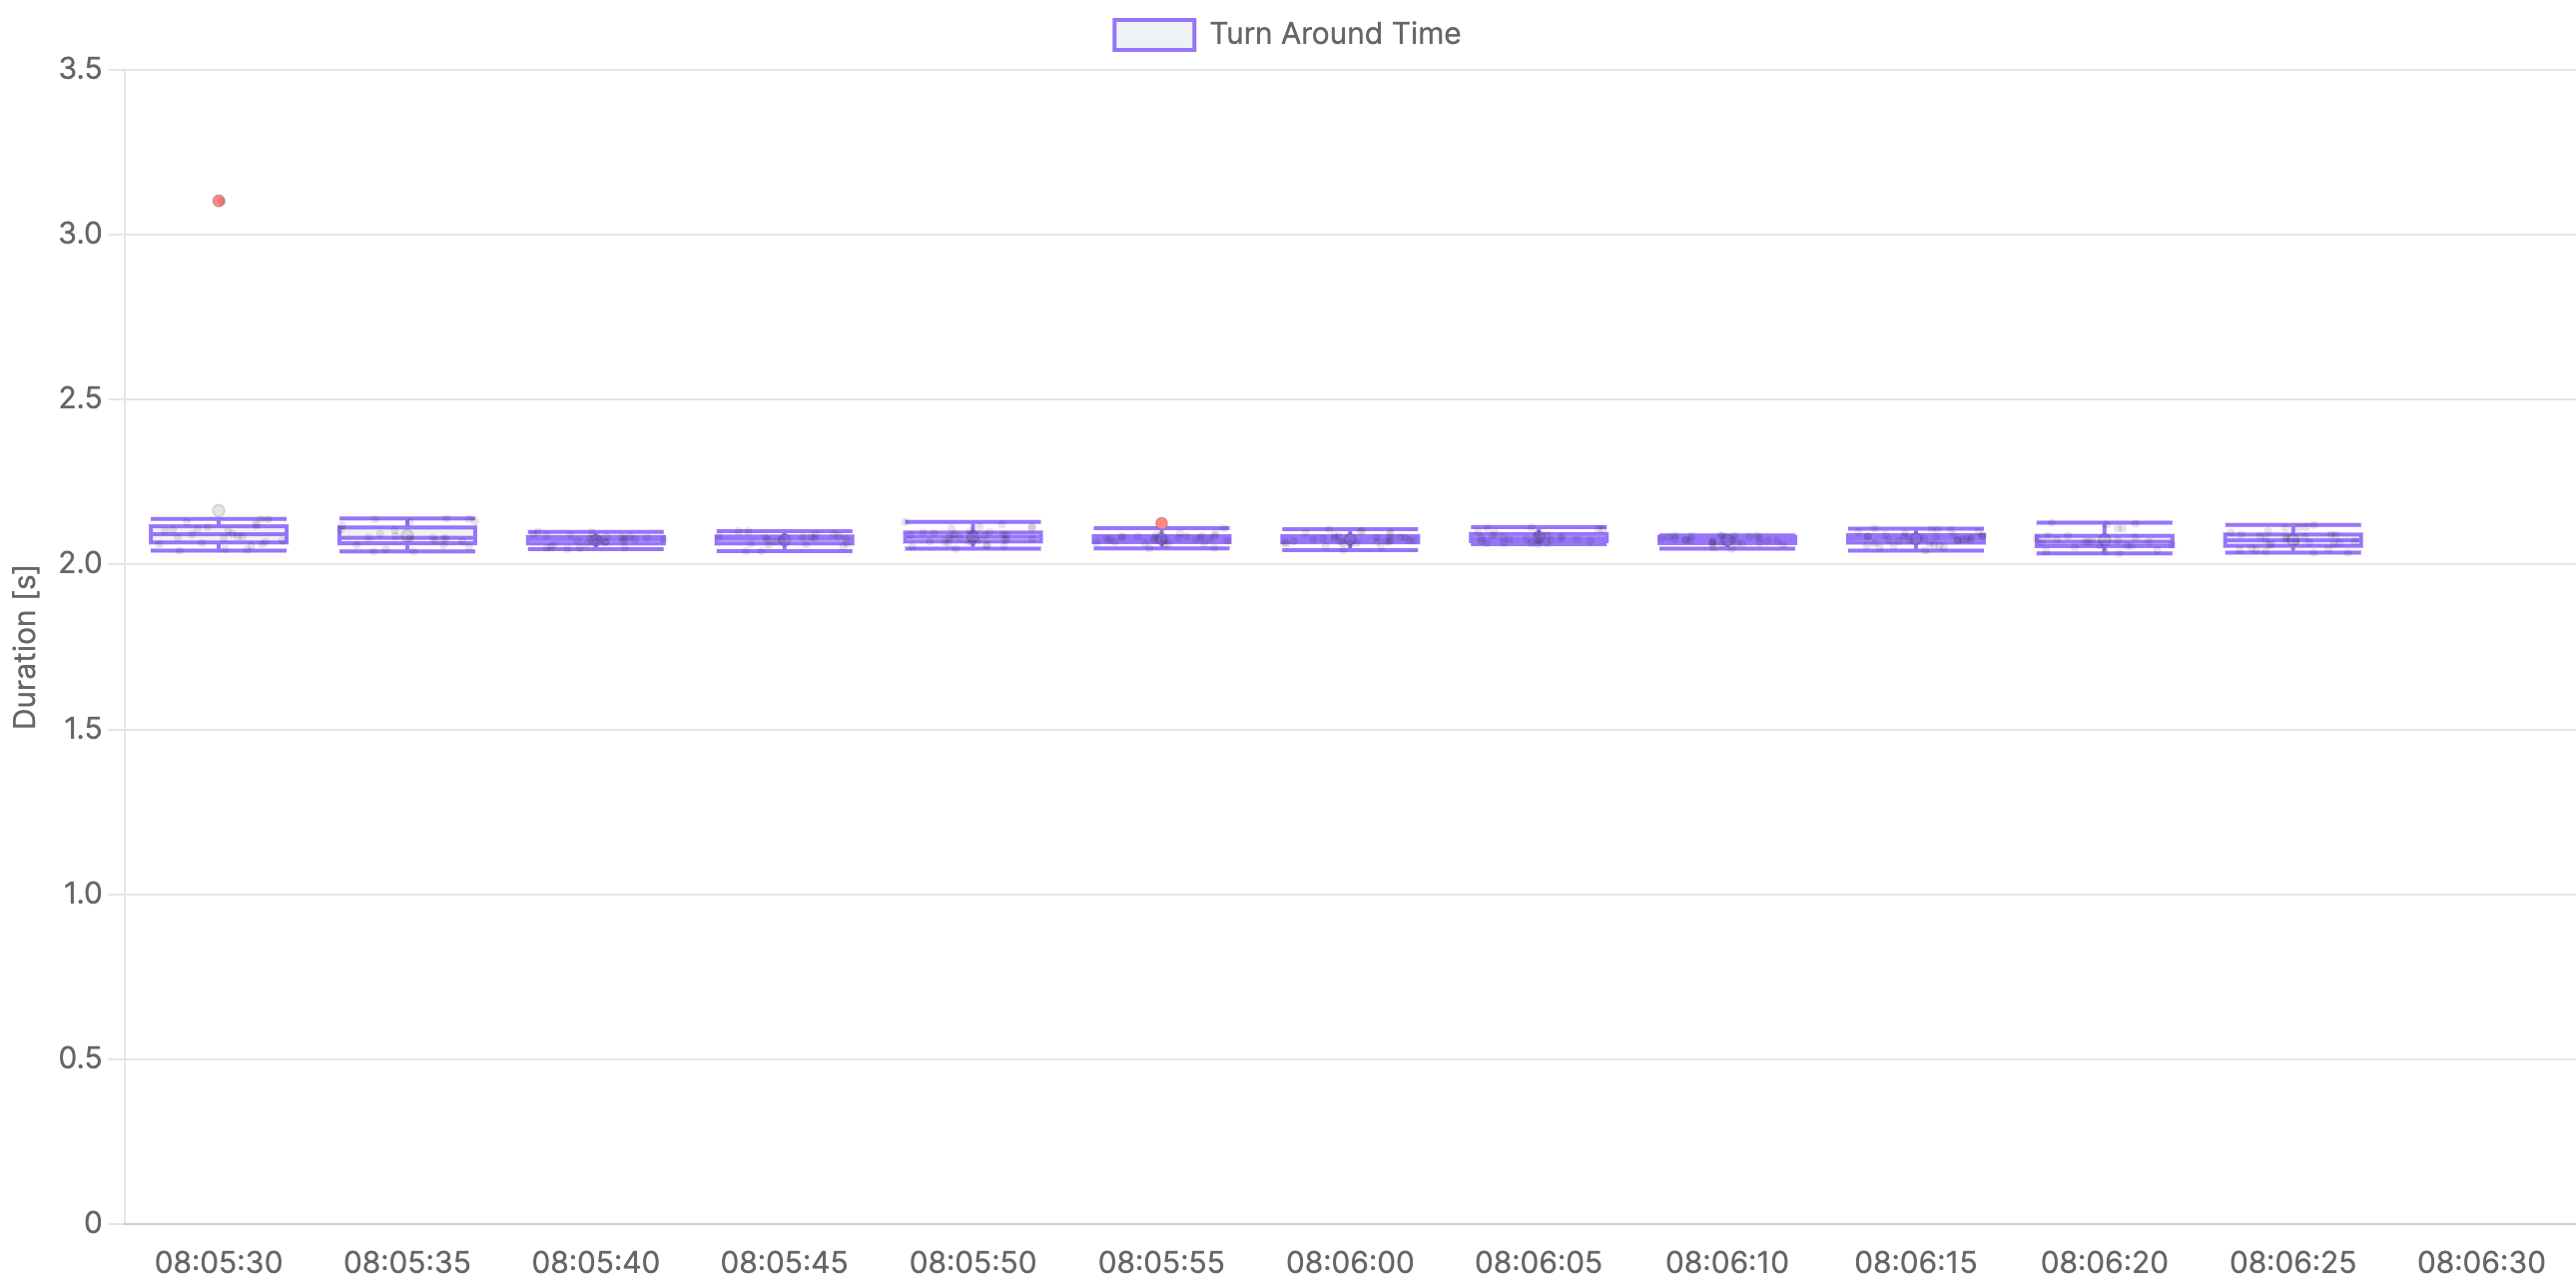
\includegraphics[width=\textwidth]{images/Judge0 FER TAT for 5 5s.png}
	\caption{
		Vrijeme obrade zahtjeva FER-ove instance sustava Judge0 za $N=5$ i $M=60$ s asinkronom interakcijom.
	}
\end{figure}
\end{frame}
\placelogotrue

\placelogofalse
\begin{frame}
\frametitle{Primjer korištenja aplikacije Hélory}
\framesubtitle{Analiza performansi FER-ove instance sustava Judge0 (2)}
\begin{figure}[htb]
	\centering
	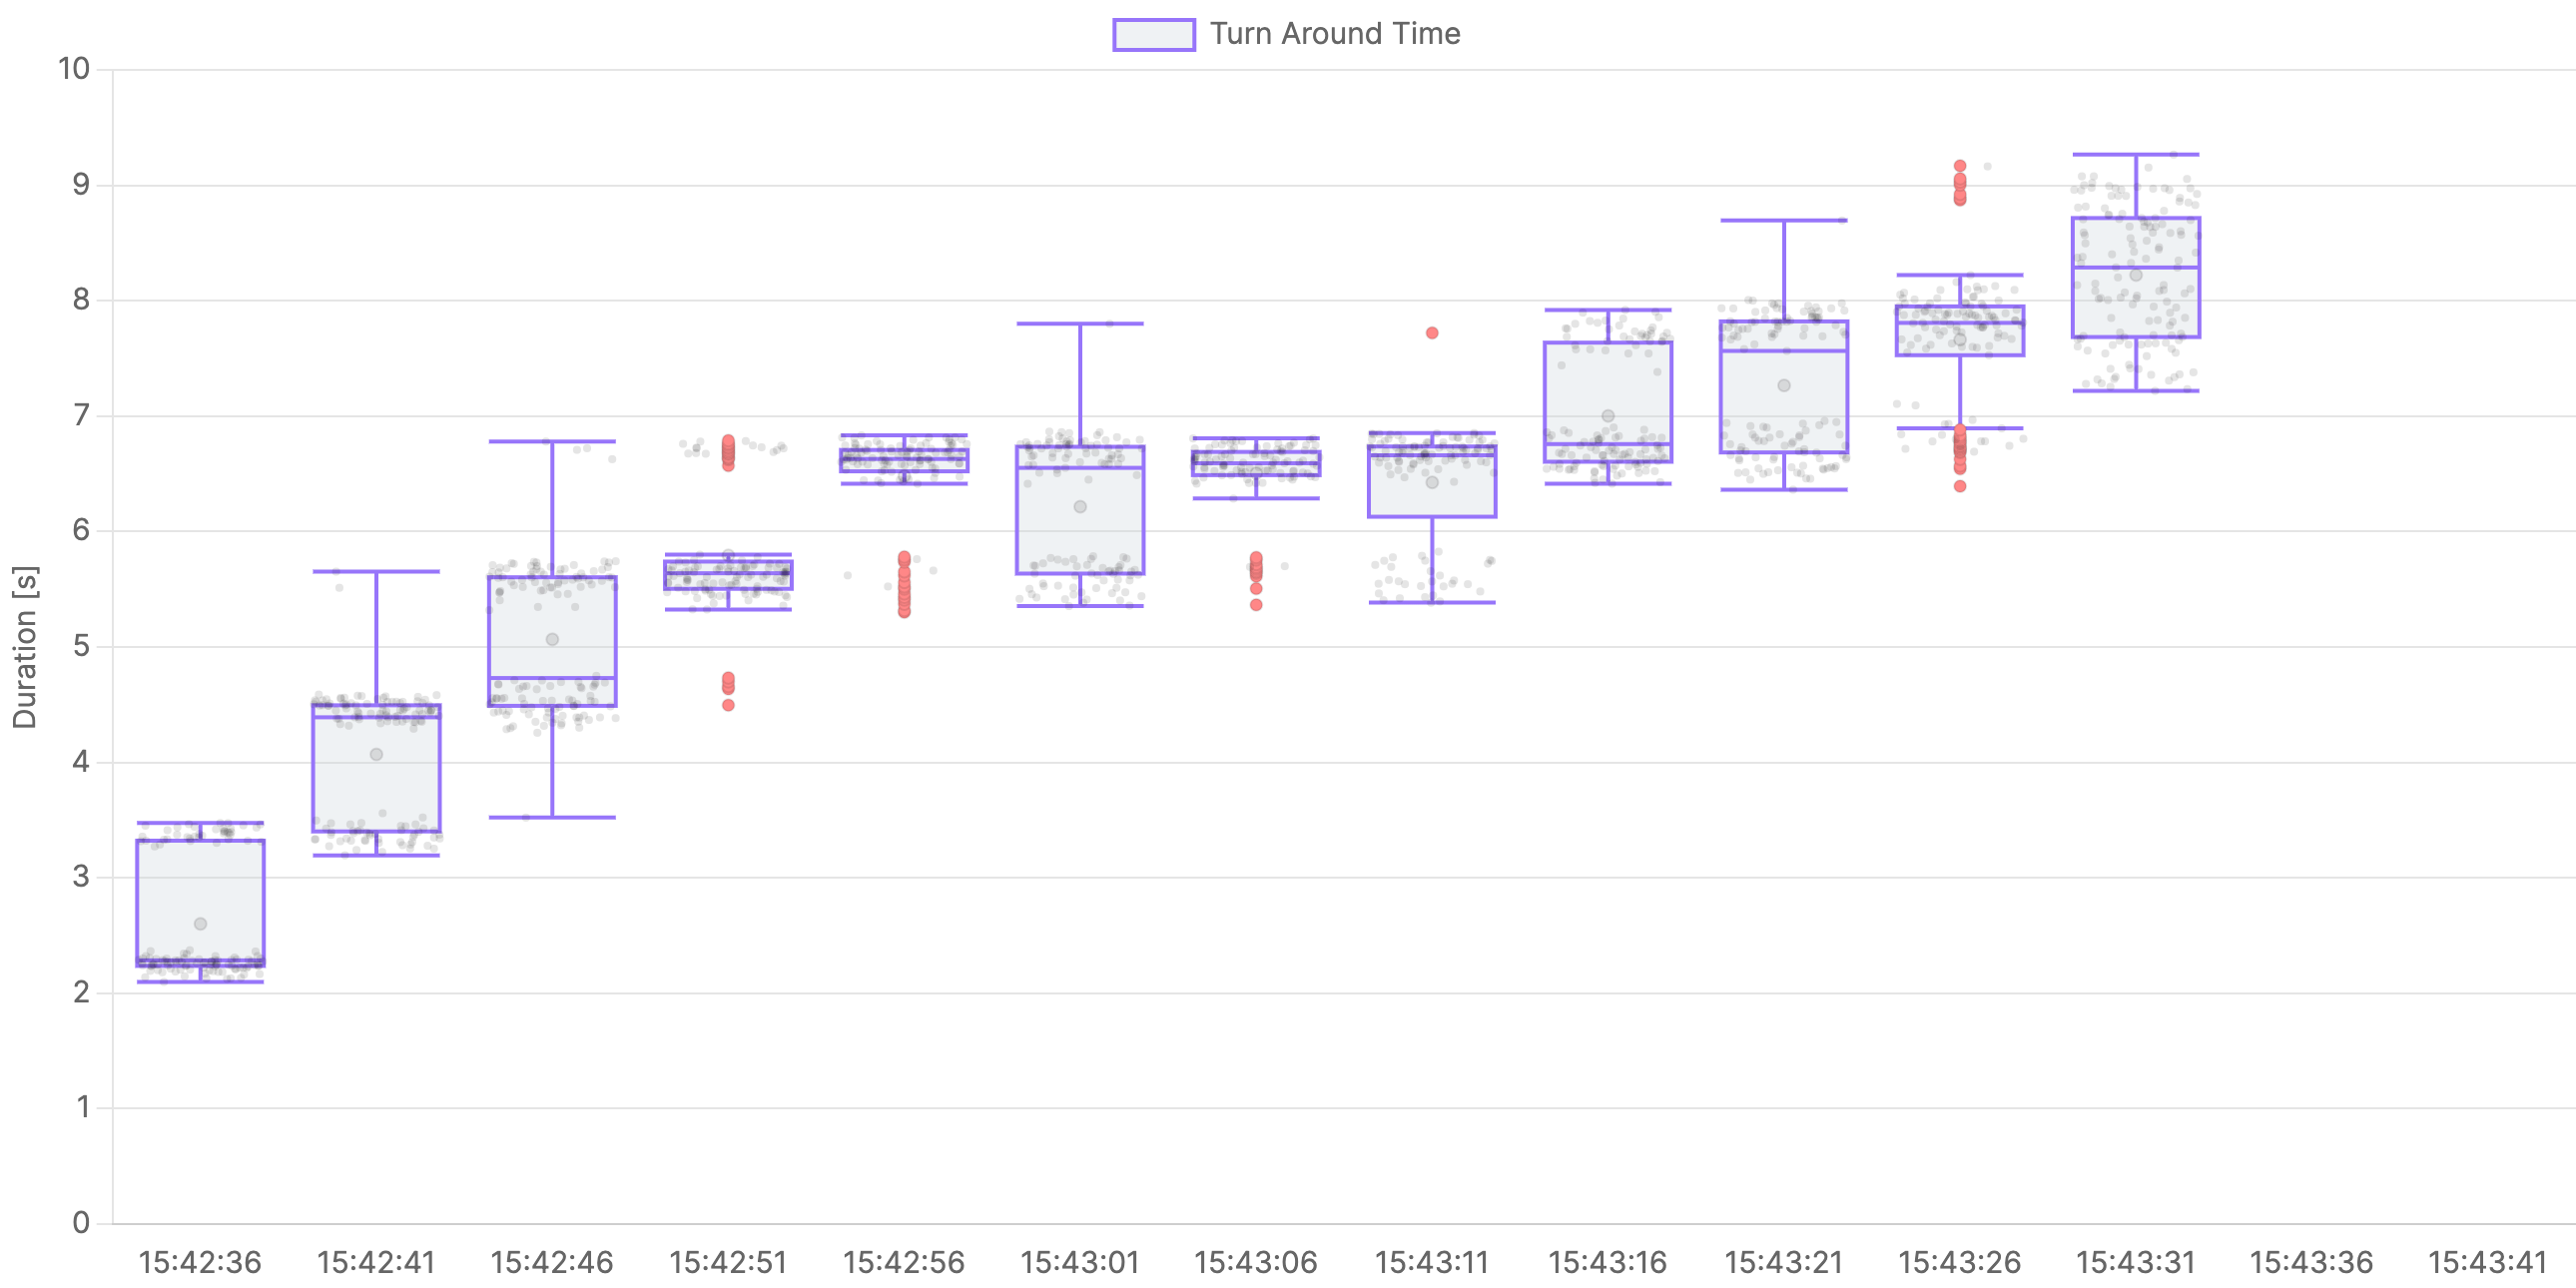
\includegraphics[width=0.89\textwidth]{images/Judge0 FER TAT for 25 5s.png}
	\caption{
		Vrijeme obrade zahtjeva FER-ove instance sustava Judge0 za $N=25$ i $M=60$ s asinkronom interakcijom.
	}
\end{figure}
\end{frame}
\placelogotrue

\placelogofalse
\begin{frame}
\frametitle{Primjer korištenja aplikacije Hélory}
\framesubtitle{Analiza performansi FER-ove instance sustava Judge0 (3)}
\begin{itemize}
	\item uspješnost obrade: 70,21\%
\end{itemize}
\begin{figure}[htb]
	\centering
	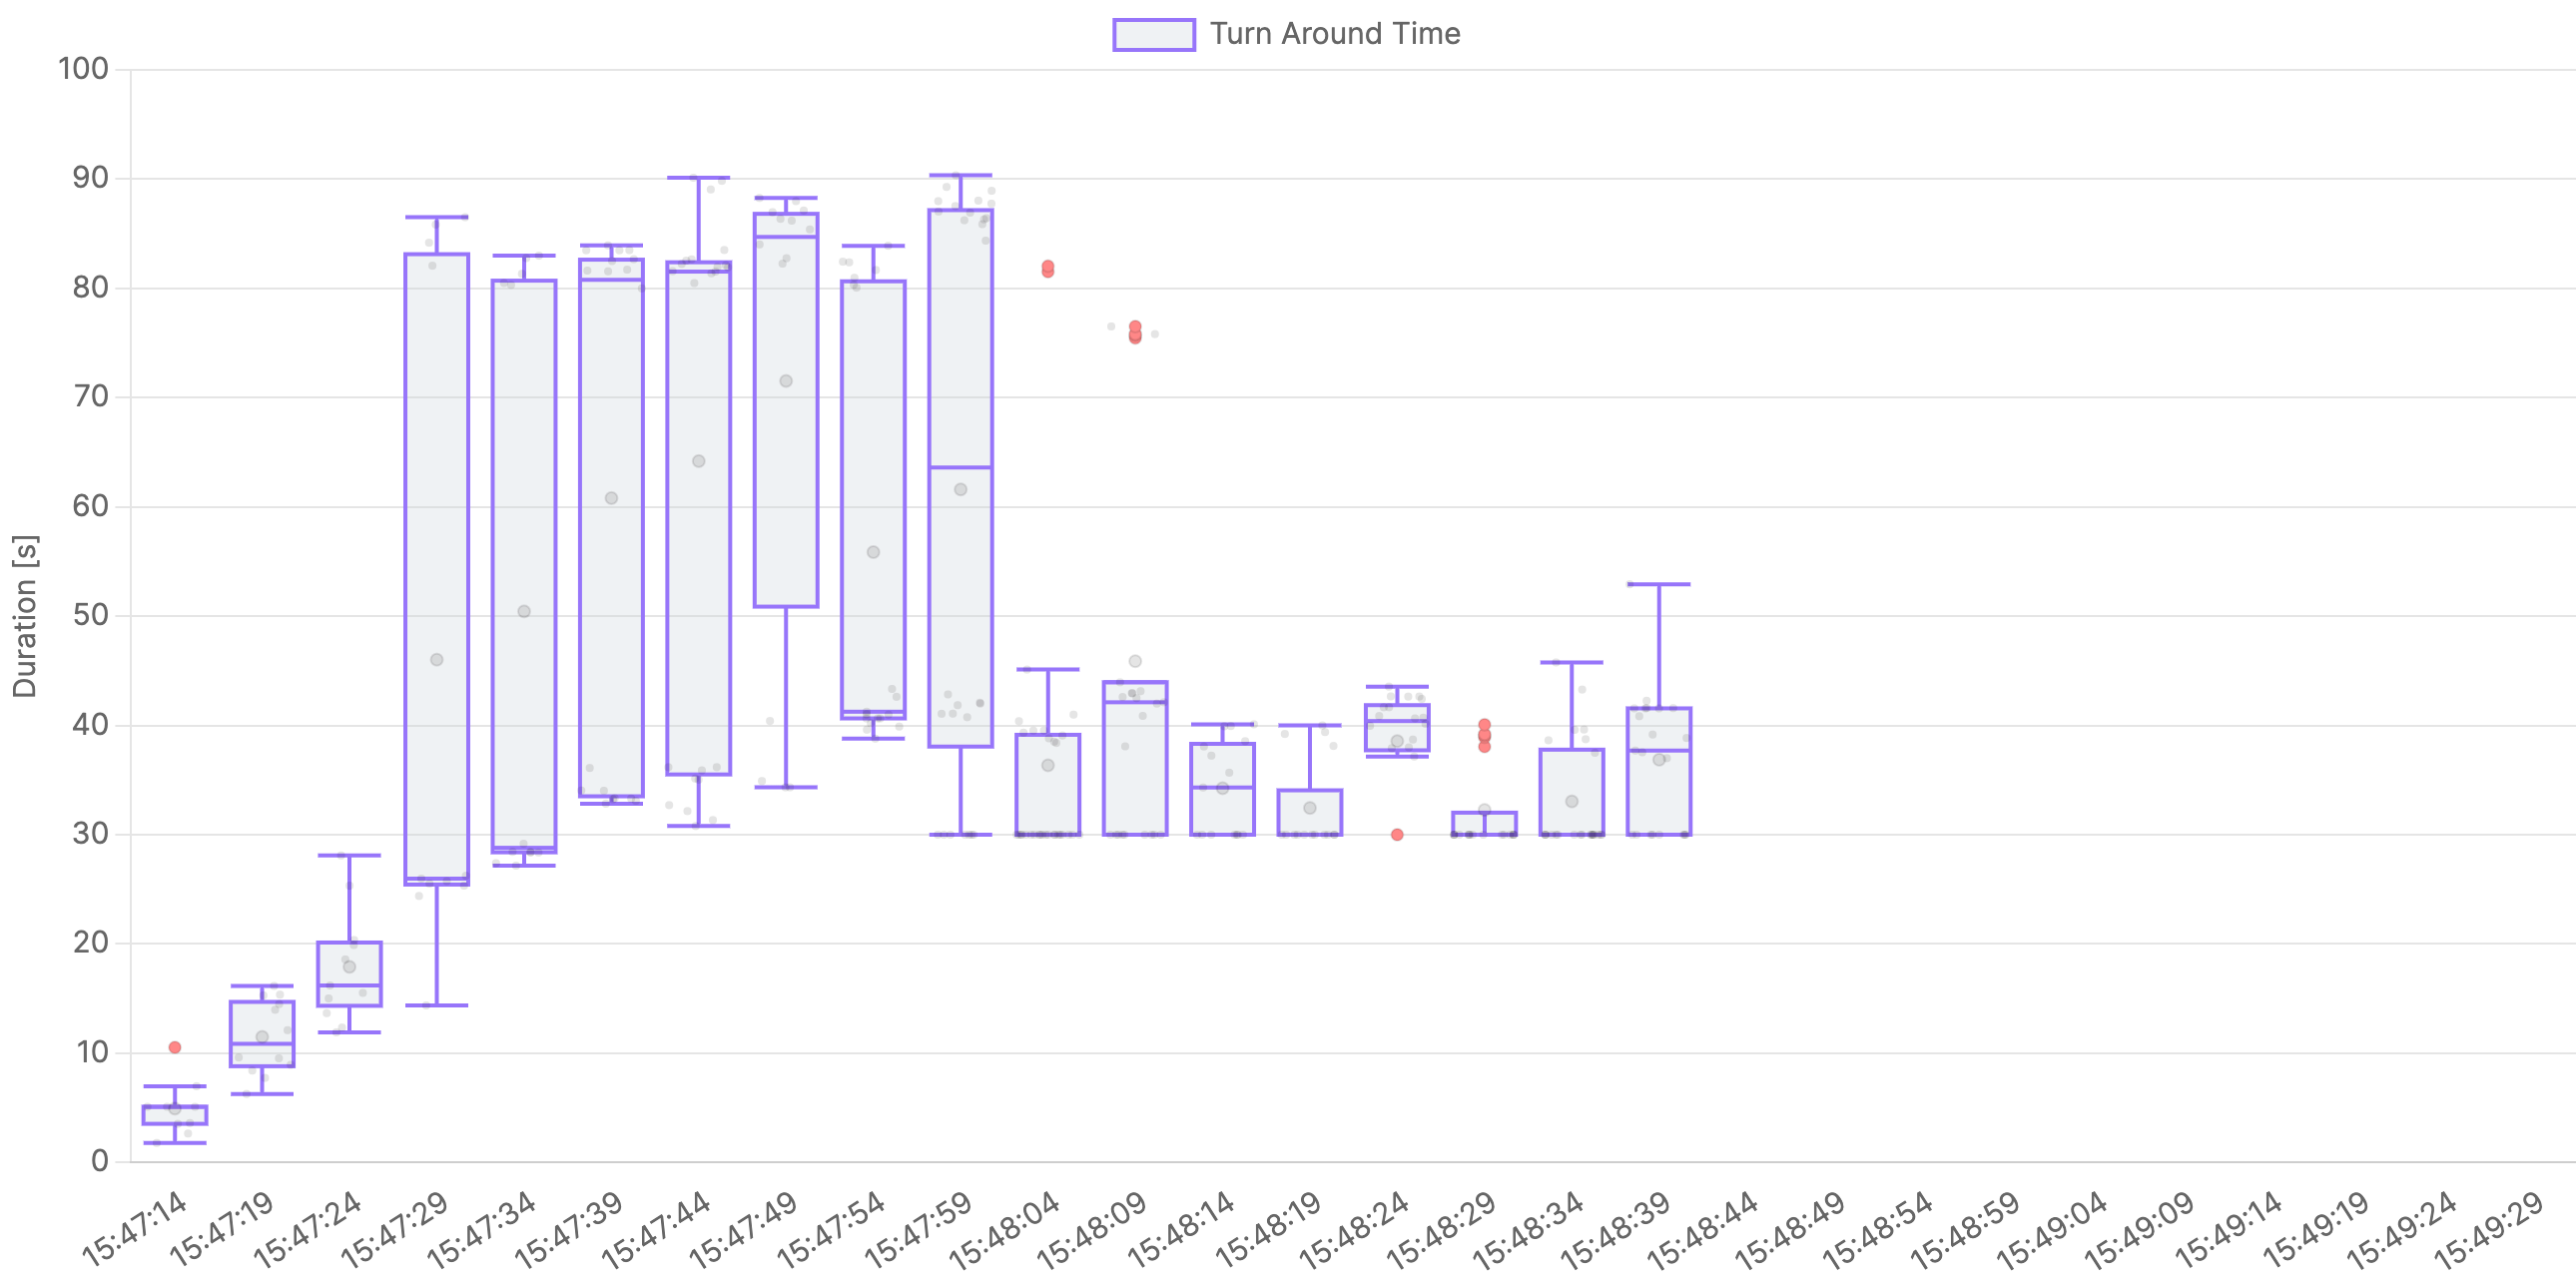
\includegraphics[width=\textwidth]{images/Judge0 FER TAT for sync 5 5s.png}
	\caption{
		Vrijeme obrade zahtjeva FER-ove instance sustava Judge0 za $N=5$ i $M=60$ sa sinkronom interakcijom.
	}
\end{figure}
\end{frame}
\placelogotrue

\placelogofalse
\begin{frame}
\frametitle{Primjer korištenja aplikacije Hélory}
\framesubtitle{Analiza performansi FER-ove instance sustava Judge0 (4)}
\begin{figure}[htb]
	\centering
	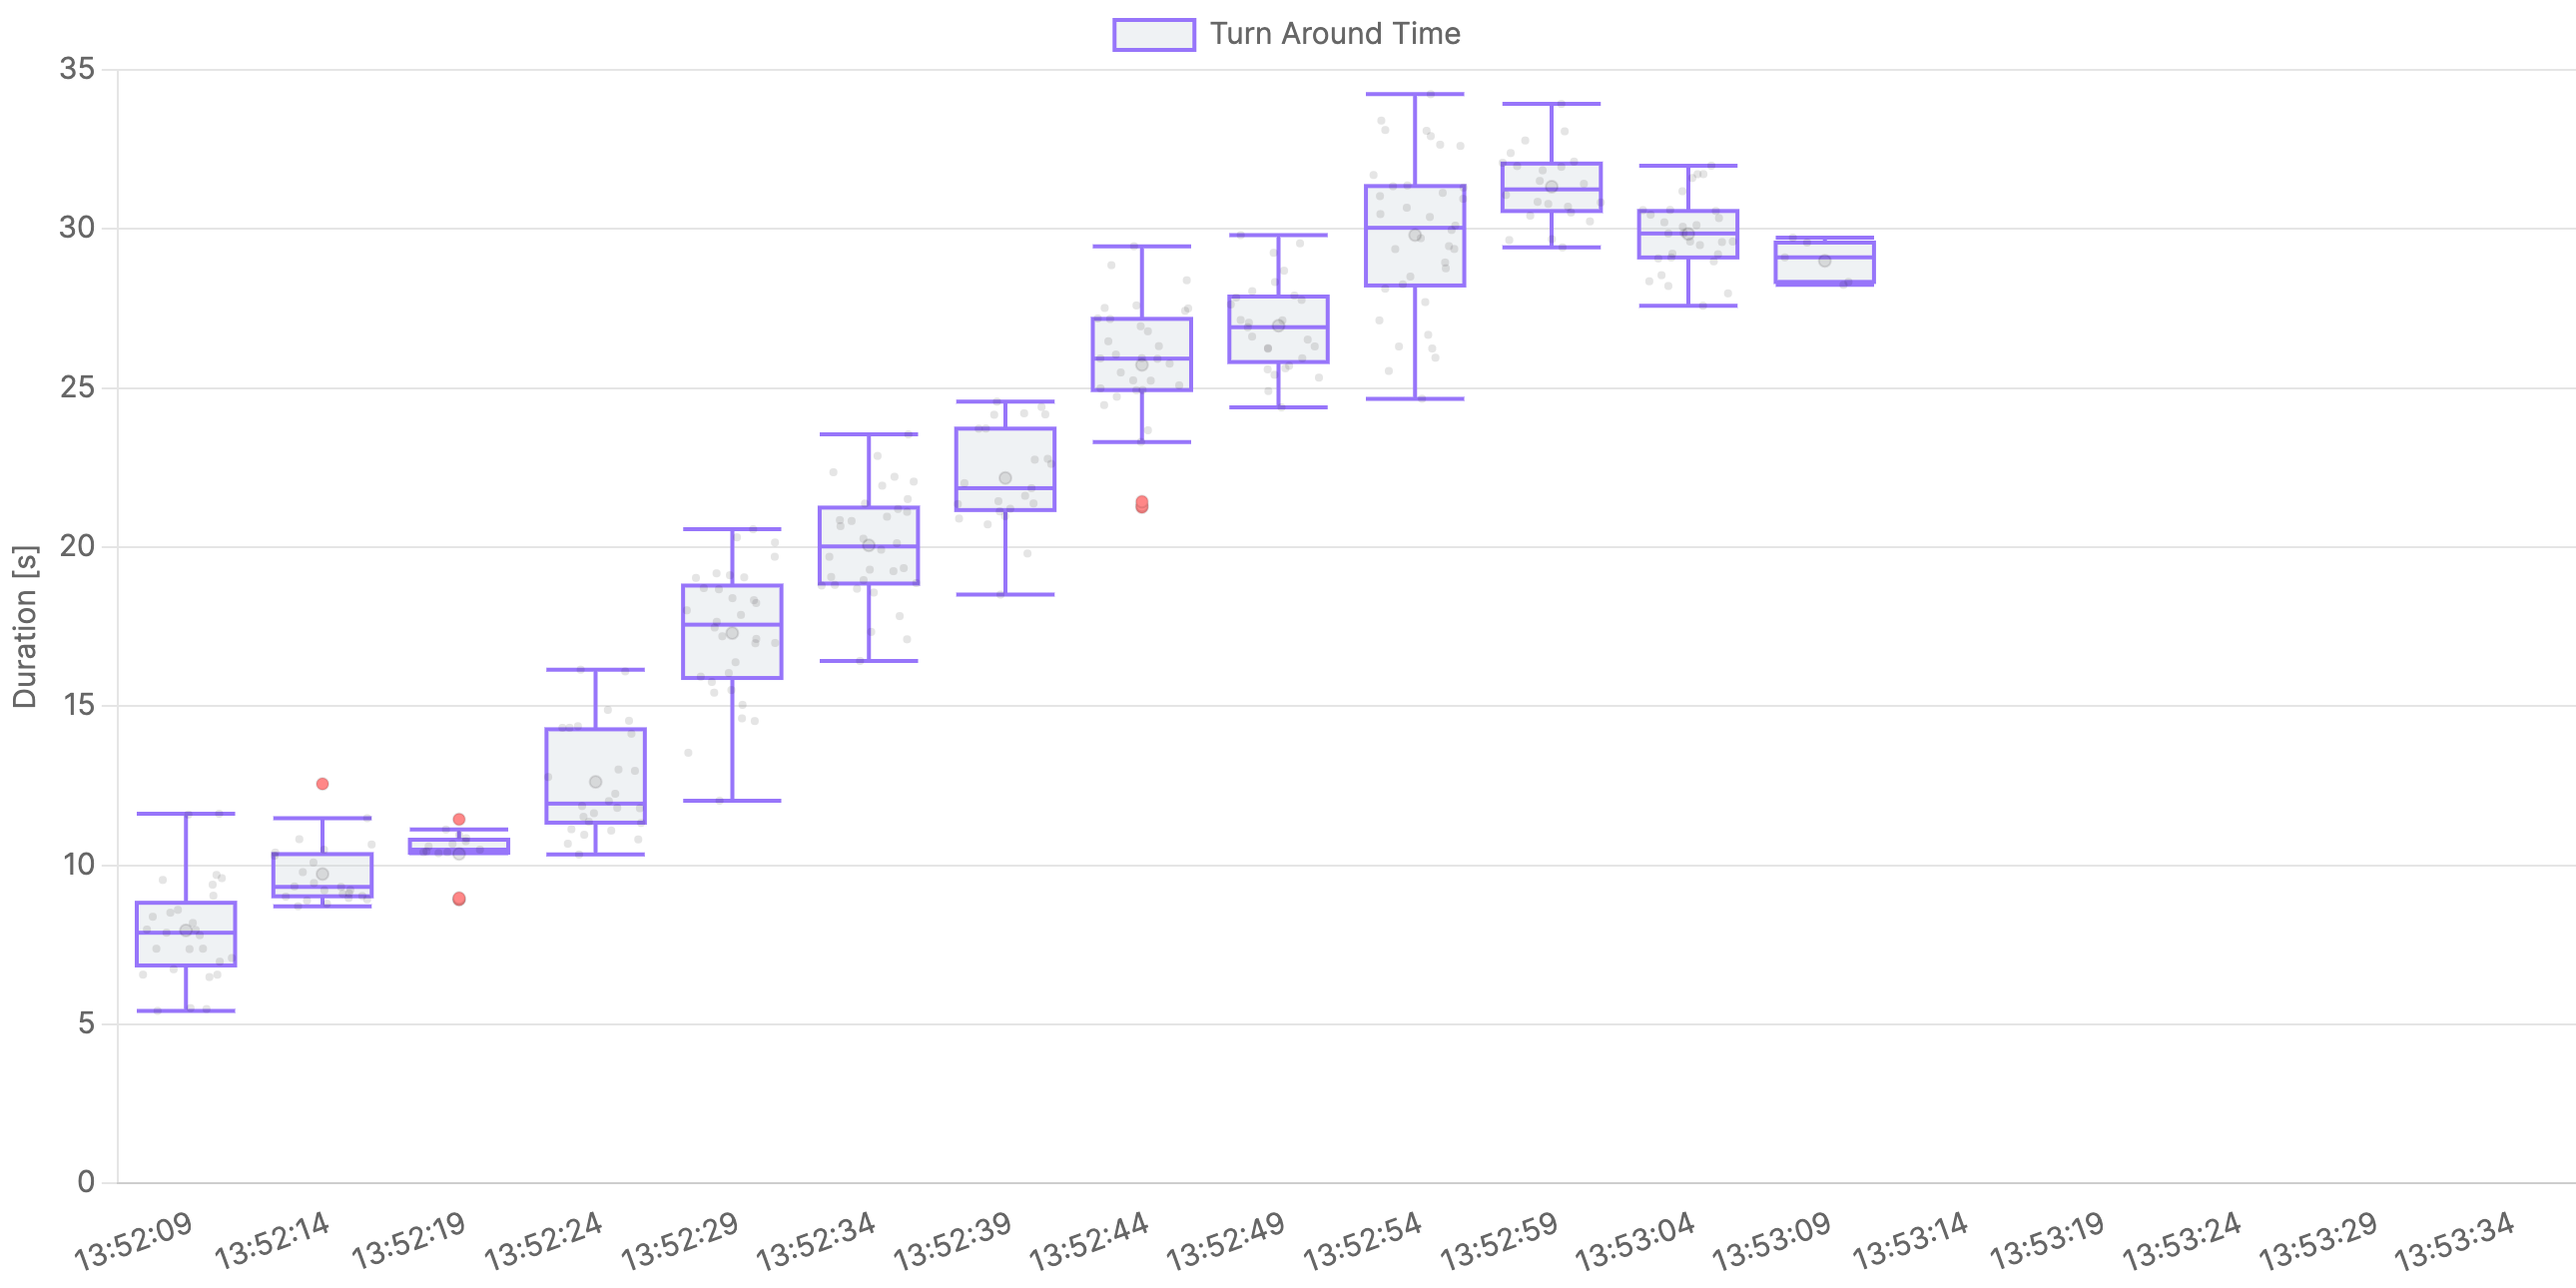
\includegraphics[width=\textwidth]{images/Judge0 FER TAT for CPU Intensive Java 5x60 5s.png}
	\caption{
		Vrijeme obrade zahtjeva FER-ove instance sustava Judge0 za $N=5$ i $M=60$ scenarija procesorskog opterećenja u Java implementaciji.
	}
\end{figure}
\end{frame}
\placelogotrue

\begin{frame}
\frametitle{Primjer korištenja aplikacije Hélory}
\framesubtitle{Analiza performansi FER-ove instance sustava Judge0 (5)}
\begin{table}[htb]
\centering
\begin{tabular}[t]{|c|c|c|}
	\hline
	\multirow{2}{*}{\bfseries Programski jezik} & 
	\multicolumn{2}{|c|}{\bfseries Scenarij korištenja}\\ \cline{2-3}
	& \lstinline{hello_world}&\lstinline{cpu_intensive} \\ \hline
	%------
	\text{C++} & 20 & 1 \\
	Java & 10 & 1 \\
	Python & 25 & 1 \\
	\hline
\end{tabular}
\caption{Maksimalno opterećenje koje podnosi FER-ova instanca sustava Judge0.}
\end{table}
\end{frame}

\section{Zaključak}
\begin{frame}
\frametitle{Zaključak}
\begin{itemize}
	\item OCES-i imaju ključni utjecaj na korisničko iskustvo.
	\item Prvi \textbf{radni okvir} za analizu performansi i ocjenu kvalitete i pouzdanosti usluge koju nude OCES-i.
	\item Aplikacija \textbf{Hélory} koja implementira predstavljeni radni okvir.
	\item Eksperimentalno je pokazano da se pri korištenju sustava Judge0 preporuča koristiti asinkronu interakciju sa sustavom.
	\item Eksperimenti nad FER-ovom instancom sustava Judge0 pokazuju dobre rezultate.
\end{itemize}
\end{frame}

\placelogofalse
\begin{frame}
\frametitle{Literatura}
\bibliography{literatura}
\bibliographystyle{fer}
\end{frame}
\placelogotrue

\end{document}
